\documentclass[11pt]{article}
\usepackage[margin=2cm]{geometry}
\usepackage{amsmath,amssymb}
\usepackage{graphicx}
\usepackage{booktabs}
\usepackage{array}
\usepackage{xcolor}
\usepackage[breakable]{tcolorbox}
\usepackage{enumitem}
\usepackage[hidelinks]{hyperref}
\allowdisplaybreaks
\setlength{\parindent}{0pt}
\setlength{\parskip}{4pt}
\definecolor{stepc}{HTML}{1F4E9E}
\definecolor{ansc}{HTML}{0B6E4F}
\newcommand{\solstep}[2]{\par\medskip{\color{stepc}\textbf{Step #1 --- #2}}\par\nopagebreak}
\newtcolorbox{probbox}[1]{colback=white,colframe=black!55,fonttitle=\bfseries,title={#1}}
\newtcolorbox{ansbox}{breakable,colback=ansc!6,colframe=ansc,fonttitle=\bfseries,title={Answer}}
\newtcolorbox{cardbox}[1]{breakable,colback=stepc!4,colframe=stepc,fonttitle=\bfseries,title={#1}}
\graphicspath{{../../../output/lecture3/3A_diode_transfer/}}
\title{Set 3A: Diode Transfer Characteristics}
\author{ECEN 325 --- Lecture 3 (Diodes) practice set}
\date{}
\begin{document}
\maketitle

\textbf{What this set trains.} Finding $V_o$ as a function of $V_i$ for circuits with diodes, resistors and DC
references, and sketching it. One method handles every circuit: assume each diode ON or OFF, solve the linear
circuit, and keep only the assumptions that check out. Each valid assumption gives one straight piece of the
characteristic. Problems 1--6 are easy, 7--12 medium, 13--18 hard. Try each problem before looking at its solution.


\begin{cardbox}{The Lecture-3 pipeline (use it for every problem in this lecture)}
\textbf{Tools --- this is all the theory you need (plus the Lecture-1/2 tools):}
\begin{enumerate}[label=\textbf{T\arabic*},leftmargin=2.2em,itemsep=1pt]
\item \emph{Diode models.} Ideal: OFF $\Leftrightarrow V_D<0$ (open), ON $\Leftrightarrow I_D>0$ ($V_D=0$).
      Constant-voltage-drop (CVD): OFF $\Leftrightarrow V_D<0.7$\,V (open), ON $\Leftrightarrow I_D>0$ ($V_D=0.7$\,V source).
      Exponential: $I_D = I_S e^{V_D/nV_T}$, i.e. $V_D = nV_T\ln(I_D/I_S)$, $V_T\approx 25$\,mV.
\item \emph{State method.} Assume ON/OFF for every diode, solve the now-linear circuit (KCL, Lecture 2), then check
      the assumptions; each check is a condition on $V_i$. The valid states tile the $V_i$ axis.
\item \emph{Small signal.} Around a DC point $I_D$ the diode is a resistor $r_d = \frac{nV_T}{I_D}$
      (valid while $|v_d|\ll nV_T$). Capacitors: open at DC; $\frac{1}{sC}$ in AC; DC supplies are AC ground.
\item \emph{Rectifier with a filter capacitor} ($f=60$\,Hz, $T = \frac{1}{f}$ half-wave, $\frac{1}{2f}$ full-wave):
      peak $V_p=\hat V_S - (\text{diode drops in the path})$; ripple $V_r \approx V_p\frac{T}{RC}$;
      $I_{D,av} \approx I_L\left(1+\pi\sqrt{2V_p/V_r}\right)$, $I_{D,max}\approx I_L\left(1+2\pi\sqrt{2V_p/V_r}\right)$;
      PIV $=$ the largest reverse voltage a diode sees.
\end{enumerate}
\textbf{Steps:}
\begin{enumerate}[leftmargin=2.2em,itemsep=1pt]
\item \emph{Pick the model} stated in the problem.
\item \emph{Transfer characteristic:} for each ON/OFF state: replace the diodes, solve, check $\Rightarrow$ range of $V_i$;
      then join the pieces (they must meet at the breakpoints) and sketch.
\item \emph{Small signal:} DC operating point first, then $r_d$, then the AC circuit exactly as in Lectures 1--2,
      then add DC and AC.
\item \emph{Rectifiers:} peak $\to$ ripple (or $C$ for a given ripple) $\to$ diode currents $\to$ PIV $\to$ transformer ratio.
\end{enumerate}
\end{cardbox}

\section*{Problems}
\subsection*{Easy problems}
\begin{probbox}{Problem 3A.1 \hfill Easy}
For the circuit below, use the constant-voltage-drop model ($V_{D,on}=0.7$\,V). Find $V_o$ as a function of $V_i$ and sketch $V_o$ versus $V_i$. Also sketch $V_o(t)$ for $V_i(t) = 5\sin(2\pi\cdot 60\,t)$.
\begin{center}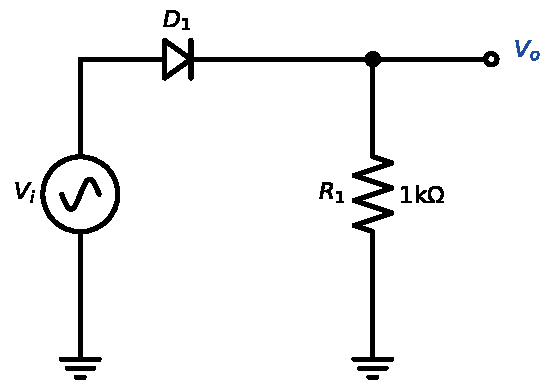
\includegraphics[width=\linewidth,height=5.6cm,keepaspectratio]{p01_circuit}\end{center}
\end{probbox}

\begin{probbox}{Problem 3A.2 \hfill Easy}
For the circuit below, use the constant-voltage-drop model ($V_{D,on}=0.7$\,V). Find $V_o$ as a function of $V_i$ and sketch $V_o$ versus $V_i$. Also sketch $V_o(t)$ for $V_i(t) = 3\sin(2\pi\cdot 1000\,t)$.
\begin{center}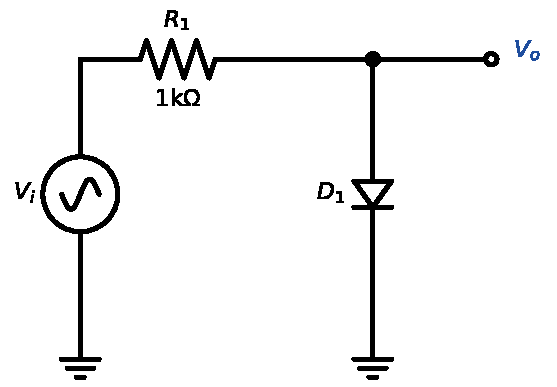
\includegraphics[width=\linewidth,height=5.6cm,keepaspectratio]{p02_circuit}\end{center}
\end{probbox}

\begin{probbox}{Problem 3A.3 \hfill Easy}
For the circuit below, use the ideal-diode model. Find $V_o$ as a function of $V_i$ and sketch $V_o$ versus $V_i$. Also sketch $V_o(t)$ for $V_i(t) = 4\sin(2\pi\cdot 1000\,t)$.
\begin{center}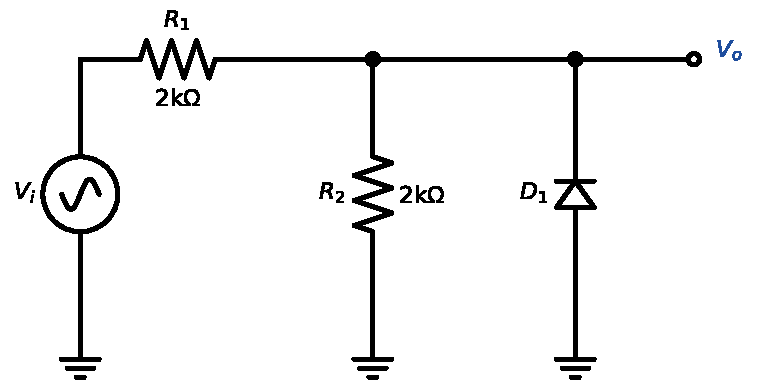
\includegraphics[width=\linewidth,height=5.6cm,keepaspectratio]{p03_circuit}\end{center}
\end{probbox}

\begin{probbox}{Problem 3A.4 \hfill Easy}
For the circuit below, use the constant-voltage-drop model ($V_{D,on}=0.7$\,V). Find $V_o$ as a function of $V_i$ and sketch $V_o$ versus $V_i$. Also sketch $V_o(t)$ for $V_i(t) = 5\sin(2\pi\cdot 1000\,t)$.
\begin{center}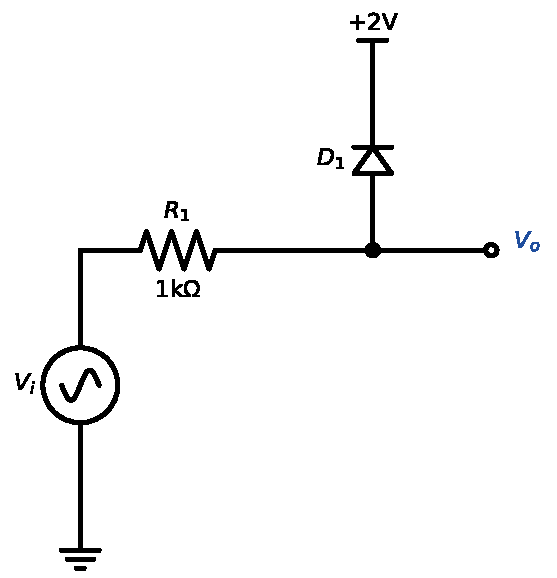
\includegraphics[width=\linewidth,height=5.6cm,keepaspectratio]{p04_circuit}\end{center}
\end{probbox}

\begin{probbox}{Problem 3A.5 \hfill Easy}
For the circuit below, use the constant-voltage-drop model ($V_{D,on}=0.7$\,V). Find $V_o$ as a function of $V_i$ and sketch $V_o$ versus $V_i$.
\begin{center}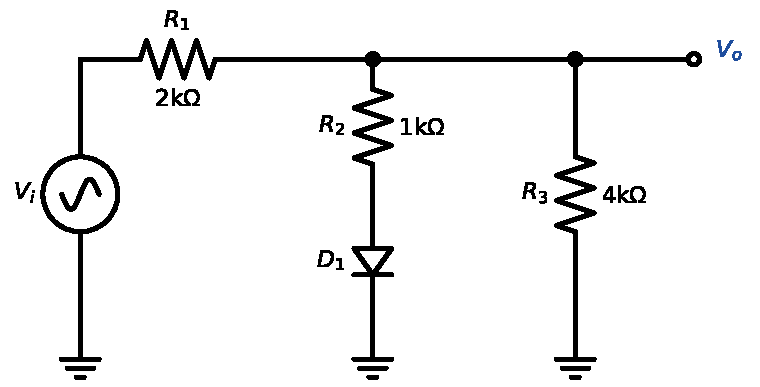
\includegraphics[width=\linewidth,height=5.6cm,keepaspectratio]{p05_circuit}\end{center}
\end{probbox}

\begin{probbox}{Problem 3A.6 \hfill Easy}
For the circuit below, use the ideal-diode model. Find $V_o$ as a function of $V_i$ and sketch $V_o$ versus $V_i$.
\begin{center}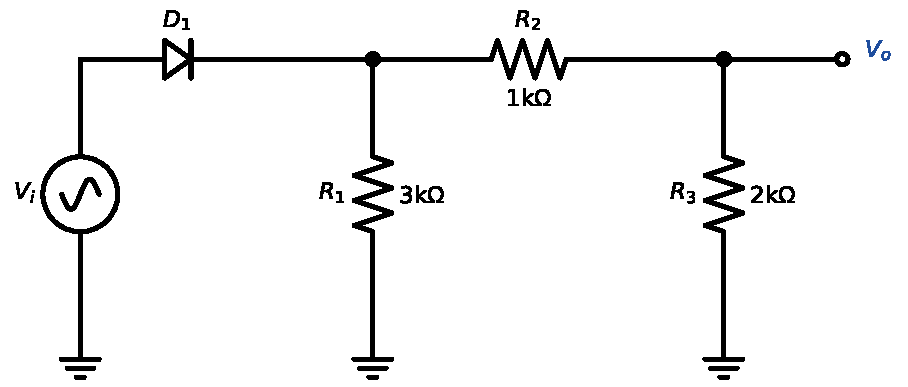
\includegraphics[width=\linewidth,height=5.6cm,keepaspectratio]{p06_circuit}\end{center}
\end{probbox}

\subsection*{Medium problems}
\begin{probbox}{Problem 3A.7 \hfill Medium}
For the circuit below, use the constant-voltage-drop model ($V_{D,on}=0.7$\,V). Find $V_o$ as a function of $V_i$ and sketch $V_o$ versus $V_i$.
\begin{center}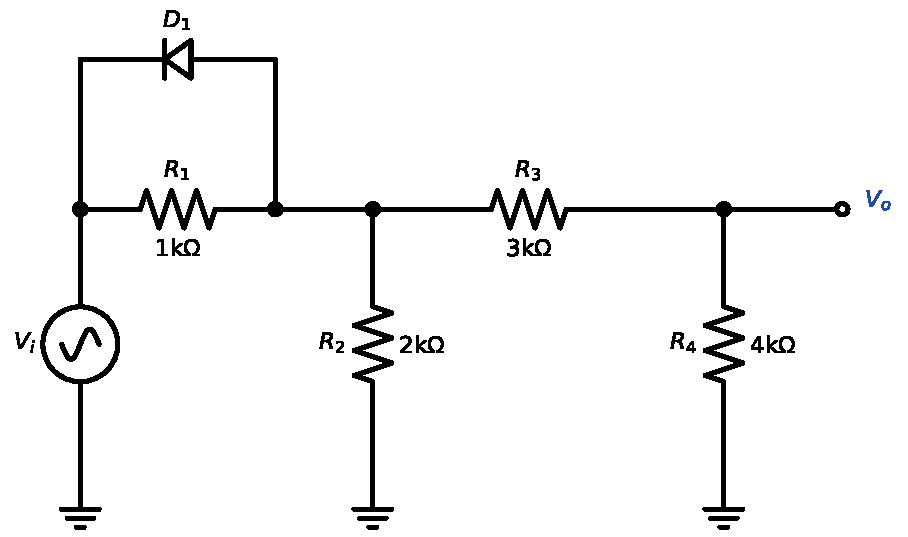
\includegraphics[width=\linewidth,height=5.6cm,keepaspectratio]{p07_circuit}\end{center}
\end{probbox}

\begin{probbox}{Problem 3A.8 \hfill Medium}
For the circuit below, use the constant-voltage-drop model ($V_{D,on}=0.7$\,V). Find $V_o$ as a function of $V_i$ and sketch $V_o$ versus $V_i$. Also sketch $V_o(t)$ for $V_i(t) = 2\sin(2\pi\cdot 1000\,t)$.
\begin{center}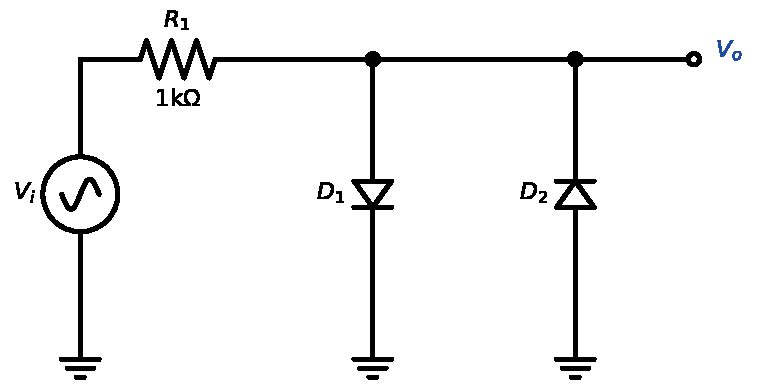
\includegraphics[width=\linewidth,height=5.6cm,keepaspectratio]{p08_circuit}\end{center}
\end{probbox}

\begin{probbox}{Problem 3A.9 \hfill Medium}
For the circuit below, use the constant-voltage-drop model ($V_{D,on}=0.7$\,V). Find $V_o$ as a function of $V_i$ and sketch $V_o$ versus $V_i$.
\begin{center}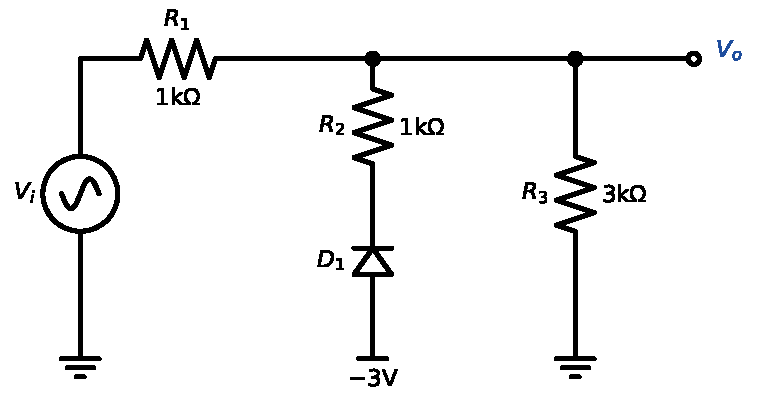
\includegraphics[width=\linewidth,height=5.6cm,keepaspectratio]{p09_circuit}\end{center}
\end{probbox}

\begin{probbox}{Problem 3A.10 \hfill Medium}
For the circuit below, use the constant-voltage-drop model ($V_{D,on}=0.7$\,V). Find $V_o$ as a function of $V_i$ and sketch $V_o$ versus $V_i$.
\begin{center}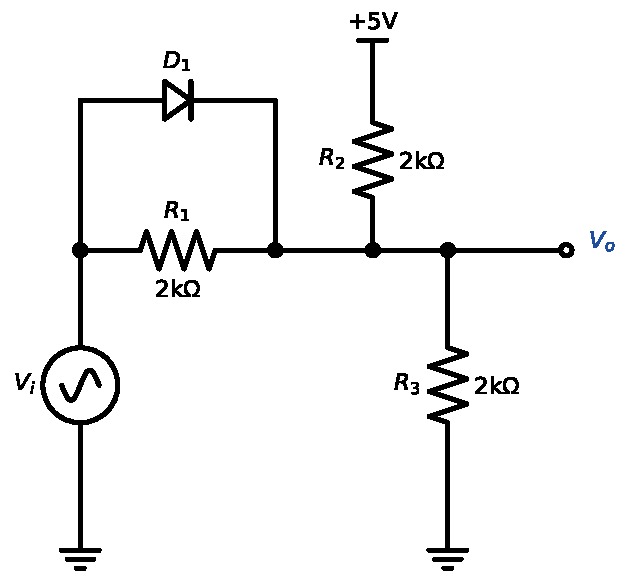
\includegraphics[width=\linewidth,height=5.6cm,keepaspectratio]{p10_circuit}\end{center}
\end{probbox}

\begin{probbox}{Problem 3A.11 \hfill Medium}
For the circuit below, use the ideal-diode model. Find $V_o$ as a function of $V_i$ and sketch $V_o$ versus $V_i$. Also sketch $V_o(t)$ for $V_i(t) = 4\sin(2\pi\cdot 500\,t)$.
\begin{center}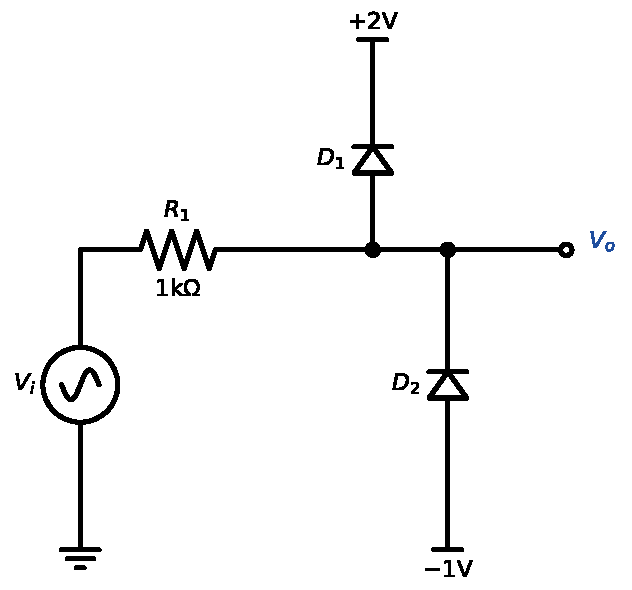
\includegraphics[width=\linewidth,height=5.6cm,keepaspectratio]{p11_circuit}\end{center}
\end{probbox}

\begin{probbox}{Problem 3A.12 \hfill Medium}
For the circuit below, use the constant-voltage-drop model ($V_{D,on}=0.7$\,V). Find $V_o$ as a function of $V_i$ and sketch $V_o$ versus $V_i$.
\begin{center}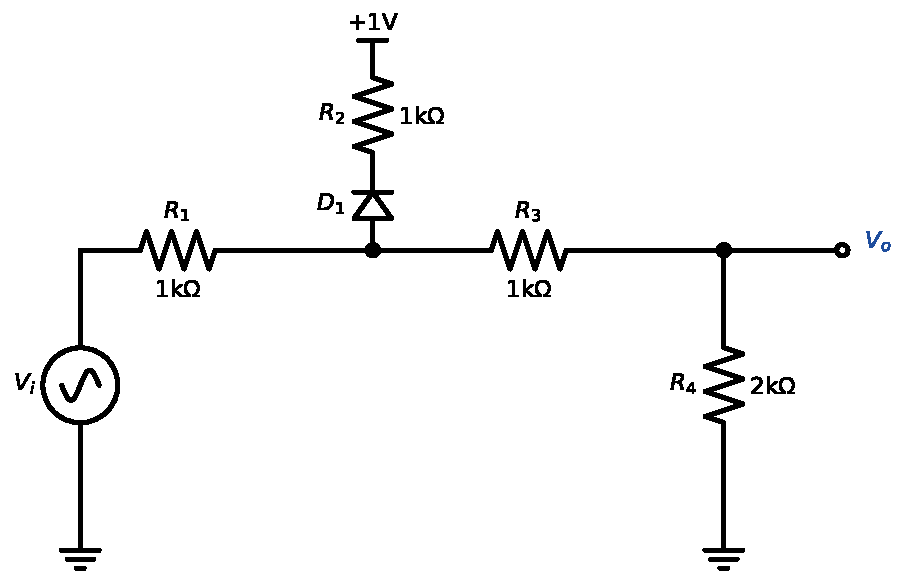
\includegraphics[width=\linewidth,height=5.6cm,keepaspectratio]{p12_circuit}\end{center}
\end{probbox}

\subsection*{Hard problems}
\begin{probbox}{Problem 3A.13 \hfill Hard}
For the circuit below, use the constant-voltage-drop model ($V_{D,on}=0.7$\,V). Find $V_o$ as a function of $V_i$ and sketch $V_o$ versus $V_i$. Also sketch $V_o(t)$ for $V_i(t) = 6\sin(2\pi\cdot 1000\,t)$.
\begin{center}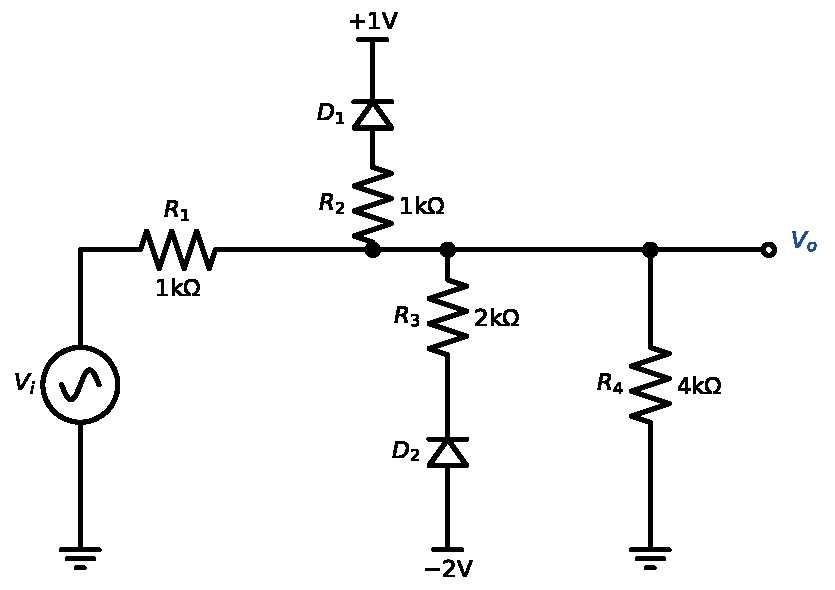
\includegraphics[width=\linewidth,height=5.6cm,keepaspectratio]{p13_circuit}\end{center}
\end{probbox}

\begin{probbox}{Problem 3A.14 \hfill Hard}
For the circuit below, use the constant-voltage-drop model ($V_{D,on}=0.7$\,V). Find $V_o$ as a function of $V_i$ and sketch $V_o$ versus $V_i$.
\begin{center}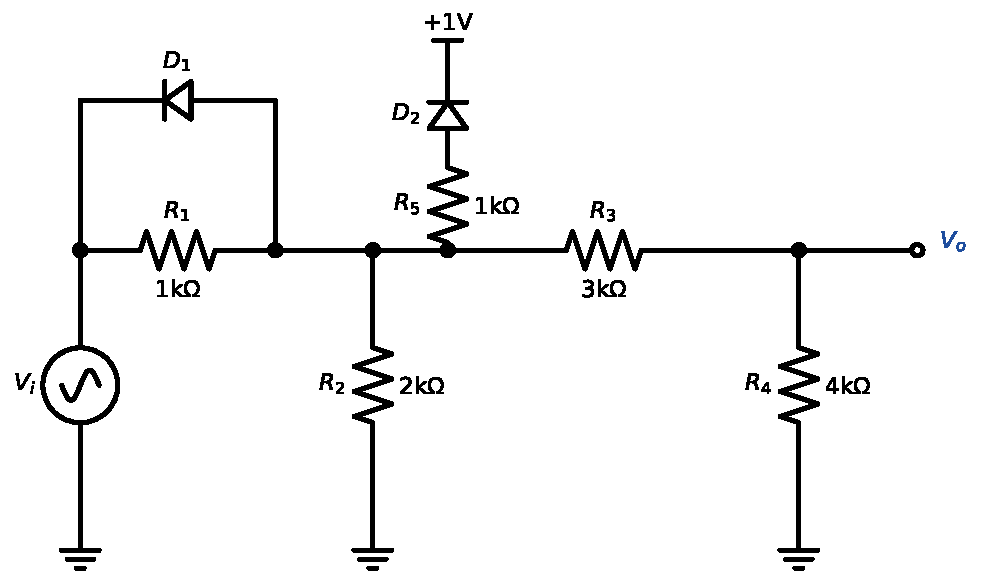
\includegraphics[width=\linewidth,height=5.6cm,keepaspectratio]{p14_circuit}\end{center}
\end{probbox}

\begin{probbox}{Problem 3A.15 \hfill Hard}
For the circuit below, use the constant-voltage-drop model ($V_{D,on}=0.7$\,V). Find $V_o$ as a function of $V_i$ and sketch $V_o$ versus $V_i$.
\begin{center}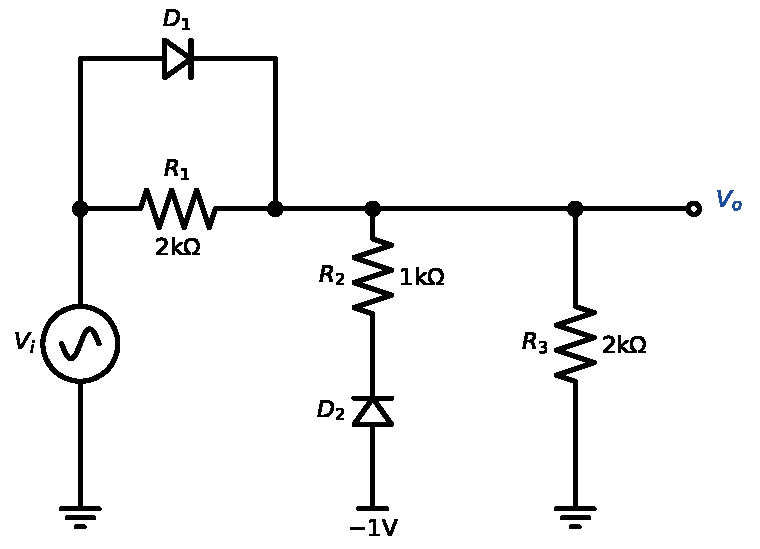
\includegraphics[width=\linewidth,height=5.6cm,keepaspectratio]{p15_circuit}\end{center}
\end{probbox}

\begin{probbox}{Problem 3A.16 \hfill Hard}
For the circuit below, use the constant-voltage-drop model ($V_{D,on}=0.7$\,V). Find $V_o$ as a function of $V_i$ and sketch $V_o$ versus $V_i$. Also sketch $V_o(t)$ for $V_i(t) = 5\sin(2\pi\cdot 1000\,t)$.
\begin{center}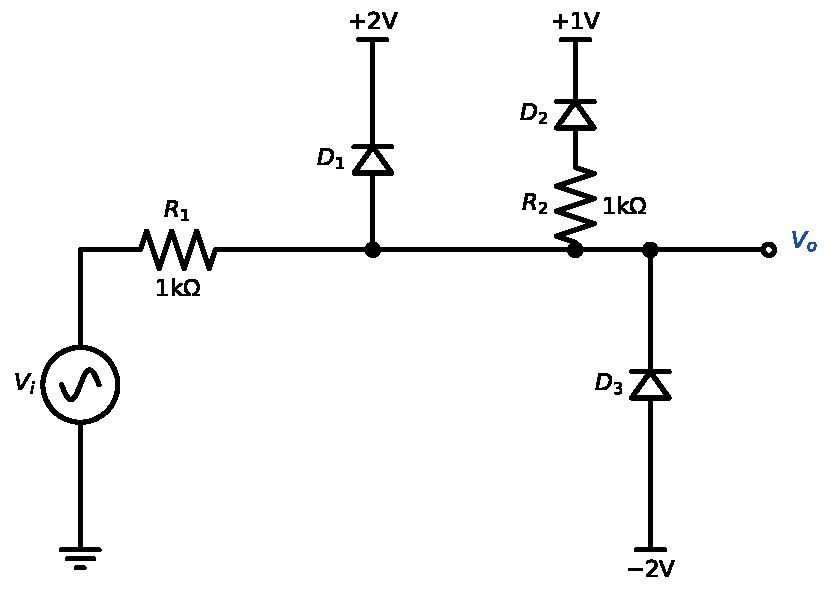
\includegraphics[width=\linewidth,height=5.6cm,keepaspectratio]{p16_circuit}\end{center}
\end{probbox}

\begin{probbox}{Problem 3A.17 \hfill Hard}
For the circuit below, use the constant-voltage-drop model ($V_{D,on}=0.7$\,V). Find $V_o$ as a function of $V_i$ and sketch $V_o$ versus $V_i$.
\begin{center}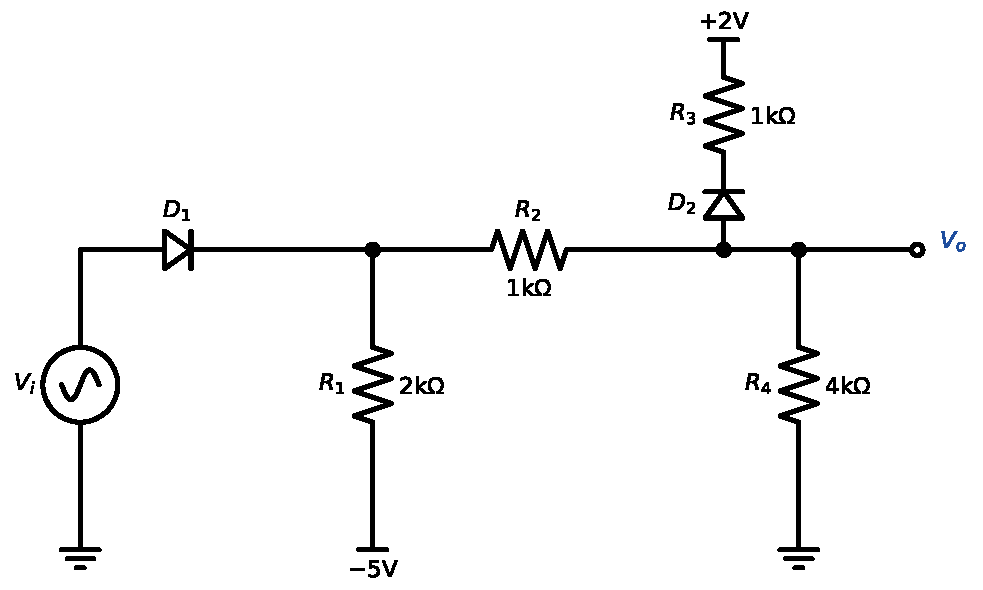
\includegraphics[width=\linewidth,height=5.6cm,keepaspectratio]{p17_circuit}\end{center}
\end{probbox}

\begin{probbox}{Problem 3A.18 \hfill Hard}
For the circuit below, use the constant-voltage-drop model ($V_{D,on}=0.7$\,V). Find $V_o$ as a function of $V_i$ and sketch $V_o$ versus $V_i$. Also sketch $V_o(t)$ for $V_i(t) = 8\sin(2\pi\cdot 1000\,t)$.
\begin{center}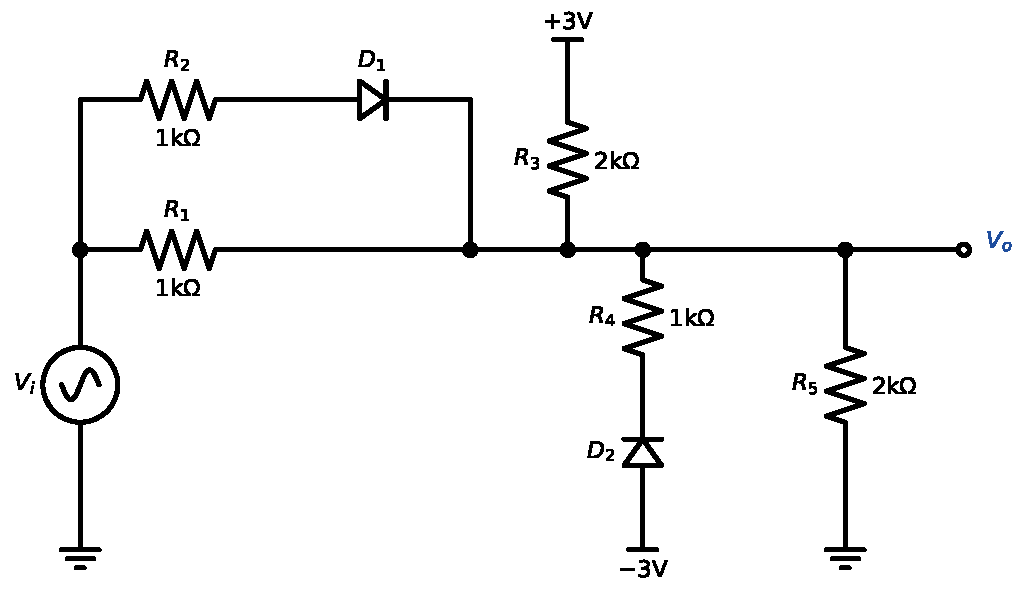
\includegraphics[width=\linewidth,height=5.6cm,keepaspectratio]{p18_circuit}\end{center}
\end{probbox}

\newpage
\section*{Solutions}
Every solution follows the steps of the Lecture-3 pipeline card.
\newpage
\subsection*{Solution 3A.1 \hfill Easy}
\begin{center}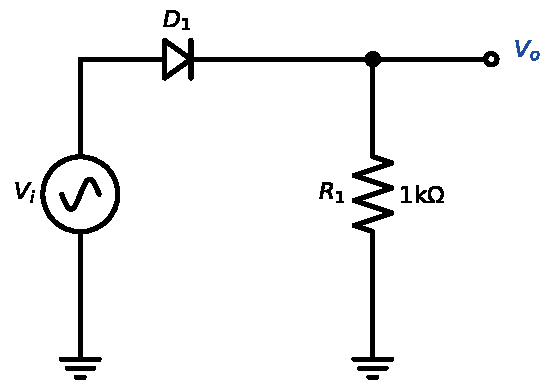
\includegraphics[width=0.9\linewidth,height=5cm,keepaspectratio]{p01_circuit}\end{center}
\solstep{1}{Model and method}Use the constant-voltage-drop model (tool T1): an OFF diode is an open circuit and needs $V_D<0.7$\,V; an ON diode is a $0.7$\,V source and needs $I_D>0$. With 1 diode there are $2$ ON/OFF combinations. For each one the circuit is linear: solve it with $V_i$ kept as a symbol, then check its assumptions --- each check is a condition on $V_i$ (tool T2).
\solstep{2}{Assume $D_{1}$ OFF}Replace $D_{1}$ OFF: an open circuit.

Equations (KCL at every node that is not an op-amp output, plus the diode voltages):\begin{align*}
&\text{KCL at }V_{o}: && \frac{V_{o}}{R_{1}} = 0
\end{align*}


Solving these linear equations (substitute one into the other, as in Lecture 2) gives, with $V_i$ kept as a symbol:\begin{align*}
V_{o} &= 0 \\
V_{D_{1}} = V_i - V_{o} &= V_i
\end{align*}


Check the assumptions: $V_{D_{1}} < 0.7$ $\Rightarrow$ $V_i < 0.7$\,V. So this state holds for $\boxed{V_i < 0.7}$, where $V_o = 0$.
\solstep{3}{Assume $D_{1}$ ON}Replace $D_{1}$ ON: a $0.7$\,V source ($V_i - V_{o} = 0.7$) carrying an unknown current $I_{D_{1}}$ from anode to cathode.

Equations (KCL at every node that is not an op-amp output, plus the diode voltages):\begin{align*}
&\text{KCL at }V_{o}: && \frac{V_{o}}{R_{1}} - I_{D_{1}} = 0 \\
&\text{D1 ON}: && V_i - V_{o} = 0.7
\end{align*}


Solving these linear equations (substitute one into the other, as in Lecture 2) gives, with $V_i$ kept as a symbol:\begin{align*}
V_{o} &= V_i - 0.7 \\
I_{D_{1}} &= V_i - 0.7\ \mathrm{mA}
\end{align*}


Check the assumptions: $I_{D_{1}} > 0$ $\Rightarrow$ $V_i > 0.7$\,V. So this state holds for $\boxed{V_i > 0.7}$, where $V_o = V_i - 0.7$.
\solstep{4}{Assemble and sketch}Put the valid states together:\[
V_o = \begin{cases} 0 & V_i < 0.7 \\ V_i - 0.7 & V_i > 0.7 \end{cases}
\]
Check: the pieces must meet at each breakpoint --- at $V_i=0.7$\,V both pieces give $V_o=0$\,V. \checkmark\begin{center}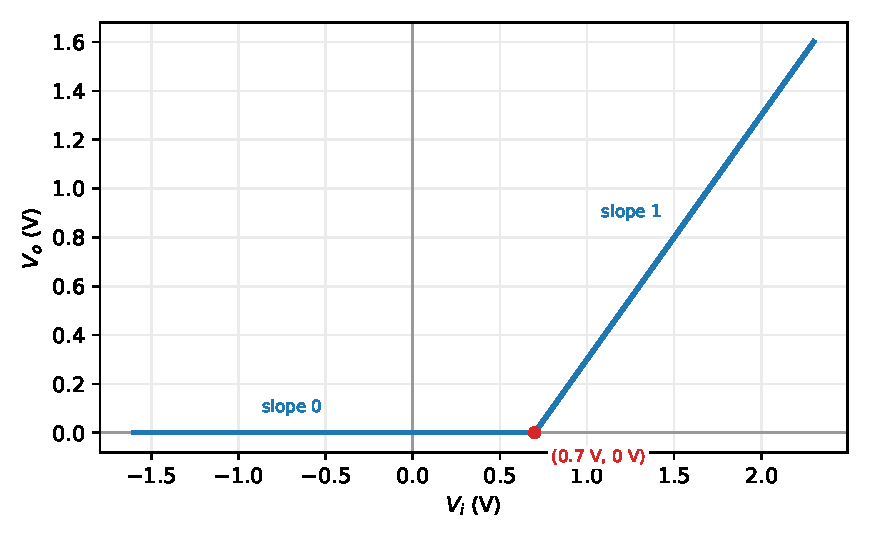
\includegraphics[width=0.62\linewidth,height=6cm,keepaspectratio]{p01_transfer}\end{center}
For $V_i(t) = 5\sin(2\pi\cdot 60\,t)$ simply pass every instant of $V_i(t)$ through the characteristic above (each piece is a straight line, so each part of the sinusoid is scaled and shifted):\begin{center}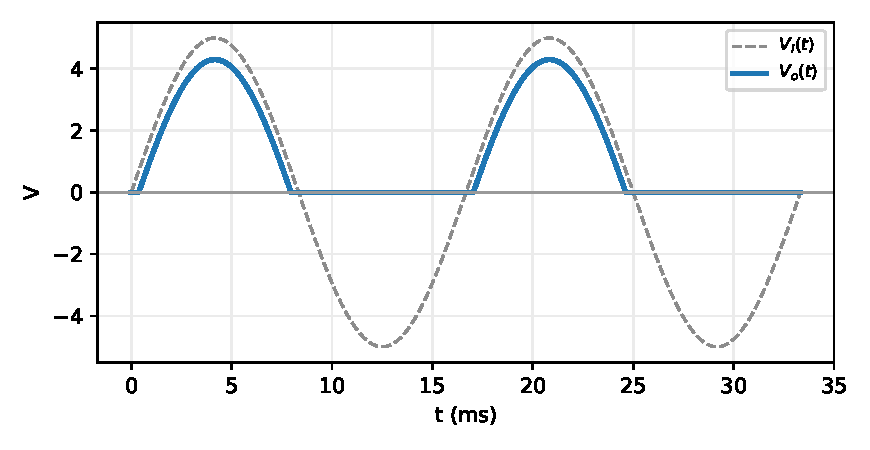
\includegraphics[width=0.62\linewidth,height=5cm,keepaspectratio]{p01_time}\end{center}

\begin{ansbox}
$V_o = \begin{cases} 0 & V_i < 0.7 \\ V_i - 0.7 & V_i > 0.7 \end{cases}$
\end{ansbox}

\newpage
\subsection*{Solution 3A.2 \hfill Easy}
\begin{center}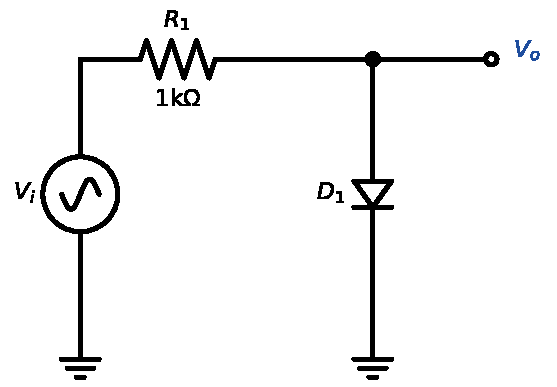
\includegraphics[width=0.9\linewidth,height=5cm,keepaspectratio]{p02_circuit}\end{center}
\solstep{1}{Model and method}Use the constant-voltage-drop model (tool T1): an OFF diode is an open circuit and needs $V_D<0.7$\,V; an ON diode is a $0.7$\,V source and needs $I_D>0$. With 1 diode there are $2$ ON/OFF combinations. For each one the circuit is linear: solve it with $V_i$ kept as a symbol, then check its assumptions --- each check is a condition on $V_i$ (tool T2).
\solstep{2}{Assume $D_{1}$ OFF}Replace $D_{1}$ OFF: an open circuit.

Equations (KCL at every node that is not an op-amp output, plus the diode voltages):\begin{align*}
&\text{KCL at }V_{o}: && \frac{V_{o} - V_i}{R_{1}} = 0
\end{align*}


Solving these linear equations (substitute one into the other, as in Lecture 2) gives, with $V_i$ kept as a symbol:\begin{align*}
V_{o} &= V_i \\
V_{D_{1}} = V_{o} - 0 &= V_i
\end{align*}


Check the assumptions: $V_{D_{1}} < 0.7$ $\Rightarrow$ $V_i < 0.7$\,V. So this state holds for $\boxed{V_i < 0.7}$, where $V_o = V_i$.
\solstep{3}{Assume $D_{1}$ ON}Replace $D_{1}$ ON: a $0.7$\,V source ($V_{o} - 0 = 0.7$) carrying an unknown current $I_{D_{1}}$ from anode to cathode.

Equations (KCL at every node that is not an op-amp output, plus the diode voltages):\begin{align*}
&\text{KCL at }V_{o}: && \frac{V_{o} - V_i}{R_{1}} + I_{D_{1}} = 0 \\
&\text{D1 ON}: && V_{o} - 0 = 0.7
\end{align*}


Solving these linear equations (substitute one into the other, as in Lecture 2) gives, with $V_i$ kept as a symbol:\begin{align*}
V_{o} &= 0.7 \\
I_{D_{1}} &= V_i - 0.7\ \mathrm{mA}
\end{align*}


Check the assumptions: $I_{D_{1}} > 0$ $\Rightarrow$ $V_i > 0.7$\,V. So this state holds for $\boxed{V_i > 0.7}$, where $V_o = 0.7$.
\solstep{4}{Assemble and sketch}Put the valid states together:\[
V_o = \begin{cases} V_i & V_i < 0.7 \\ 0.7 & V_i > 0.7 \end{cases}
\]
Check: the pieces must meet at each breakpoint --- at $V_i=0.7$\,V both pieces give $V_o=0.7$\,V. \checkmark\begin{center}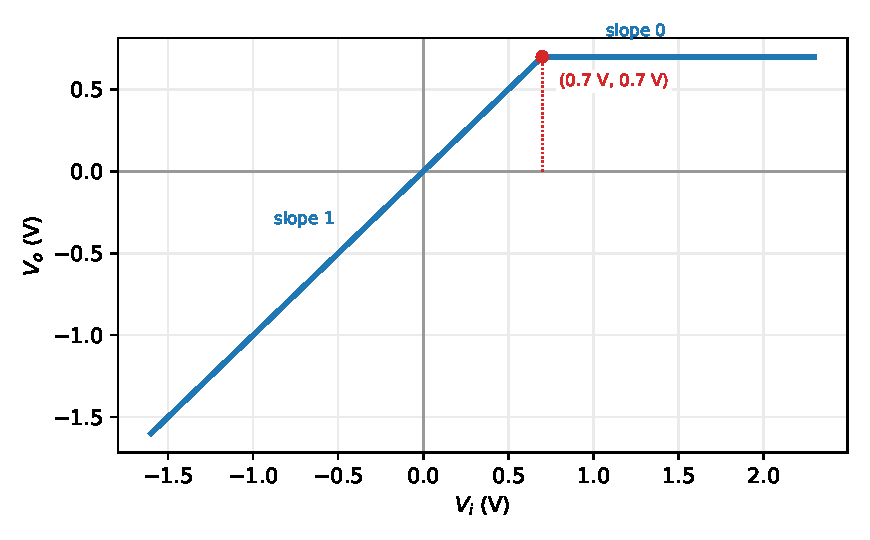
\includegraphics[width=0.62\linewidth,height=6cm,keepaspectratio]{p02_transfer}\end{center}
For $V_i(t) = 3\sin(2\pi\cdot 1000\,t)$ simply pass every instant of $V_i(t)$ through the characteristic above (each piece is a straight line, so each part of the sinusoid is scaled and shifted):\begin{center}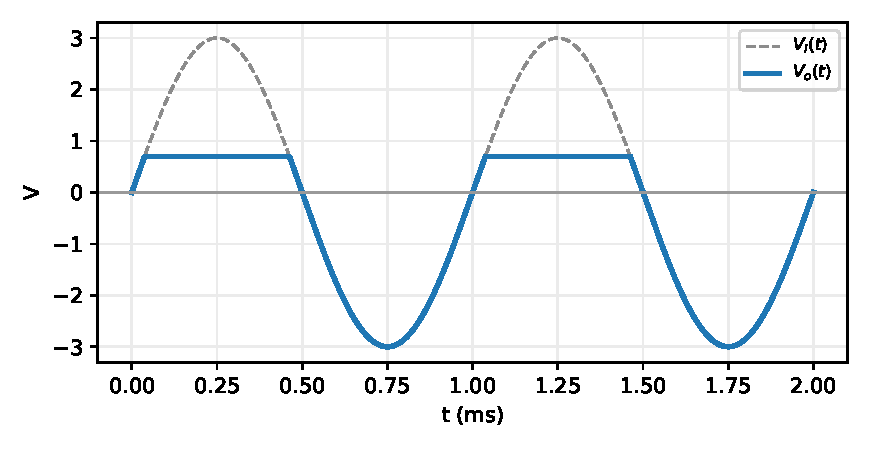
\includegraphics[width=0.62\linewidth,height=5cm,keepaspectratio]{p02_time}\end{center}

\begin{ansbox}
$V_o = \begin{cases} V_i & V_i < 0.7 \\ 0.7 & V_i > 0.7 \end{cases}$
\end{ansbox}

\newpage
\subsection*{Solution 3A.3 \hfill Easy}
\begin{center}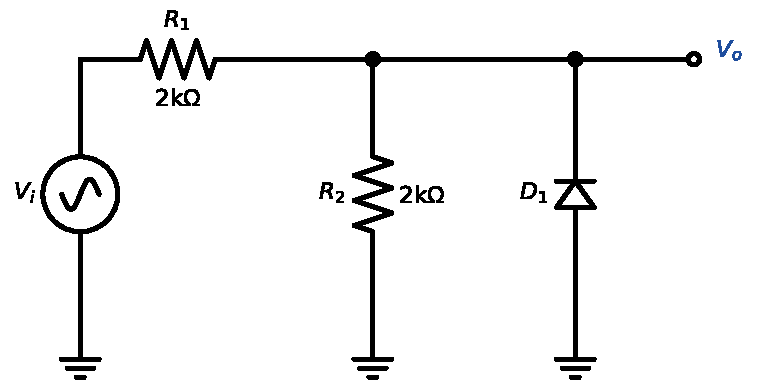
\includegraphics[width=0.9\linewidth,height=5cm,keepaspectratio]{p03_circuit}\end{center}
\solstep{1}{Model and method}Use the ideal-diode model (tool T1): an OFF diode is an open circuit and needs $V_D<0$; an ON diode is a short ($V_D=0$) and needs $I_D>0$. With 1 diode there are $2$ ON/OFF combinations. For each one the circuit is linear: solve it with $V_i$ kept as a symbol, then check its assumptions --- each check is a condition on $V_i$ (tool T2).
\solstep{2}{Assume $D_{1}$ ON}Replace $D_{1}$ ON: a $0$\,V source ($0 - V_{o} = 0$) carrying an unknown current $I_{D_{1}}$ from anode to cathode.

Equations (KCL at every node that is not an op-amp output, plus the diode voltages):\begin{align*}
&\text{KCL at }V_{o}: && \frac{V_{o} - V_i}{R_{1}} + \frac{V_{o}}{R_{2}} - I_{D_{1}} = 0 \\
&\text{D1 ON}: && 0 - V_{o} = 0
\end{align*}


Solving these linear equations (substitute one into the other, as in Lecture 2) gives, with $V_i$ kept as a symbol:\begin{align*}
V_{o} &= 0 \\
I_{D_{1}} &= -0.5V_i\ \mathrm{mA}
\end{align*}


Check the assumptions: $I_{D_{1}} > 0$ $\Rightarrow$ $V_i < 0$\,V. So this state holds for $\boxed{V_i < 0}$, where $V_o = 0$.
\solstep{3}{Assume $D_{1}$ OFF}Replace $D_{1}$ OFF: an open circuit.

Equations (KCL at every node that is not an op-amp output, plus the diode voltages):\begin{align*}
&\text{KCL at }V_{o}: && \frac{V_{o} - V_i}{R_{1}} + \frac{V_{o}}{R_{2}} = 0
\end{align*}


Solving these linear equations (substitute one into the other, as in Lecture 2) gives, with $V_i$ kept as a symbol:\begin{align*}
V_{o} &= 0.5V_i \\
V_{D_{1}} = 0 - V_{o} &= -0.5V_i
\end{align*}


Check the assumptions: $V_{D_{1}} < 0$ $\Rightarrow$ $V_i > 0$\,V. So this state holds for $\boxed{V_i > 0}$, where $V_o = 0.5V_i$.
\solstep{4}{Assemble and sketch}Put the valid states together:\[
V_o = \begin{cases} 0 & V_i < 0 \\ 0.5V_i & V_i > 0 \end{cases}
\]
Check: the pieces must meet at each breakpoint --- at $V_i=0$\,V both pieces give $V_o=0$\,V. \checkmark\begin{center}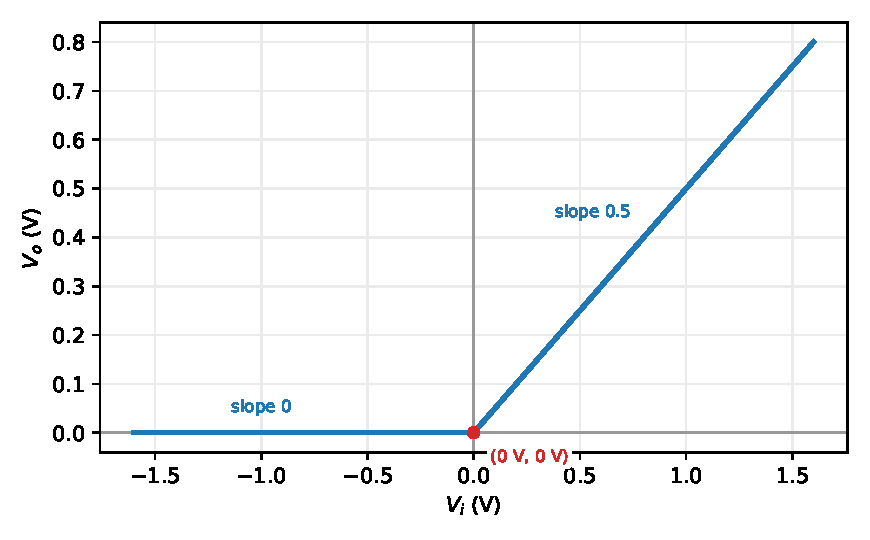
\includegraphics[width=0.62\linewidth,height=6cm,keepaspectratio]{p03_transfer}\end{center}
For $V_i(t) = 4\sin(2\pi\cdot 1000\,t)$ simply pass every instant of $V_i(t)$ through the characteristic above (each piece is a straight line, so each part of the sinusoid is scaled and shifted):\begin{center}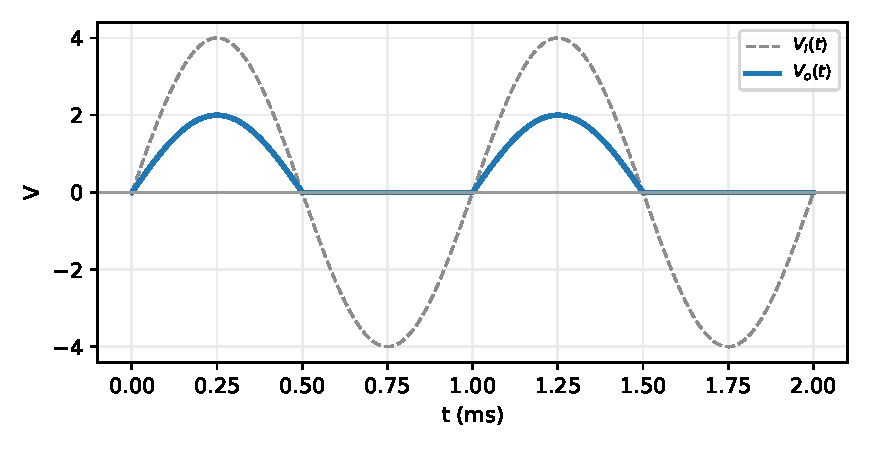
\includegraphics[width=0.62\linewidth,height=5cm,keepaspectratio]{p03_time}\end{center}

\begin{ansbox}
$V_o = \begin{cases} 0 & V_i < 0 \\ 0.5V_i & V_i > 0 \end{cases}$
\end{ansbox}

\newpage
\subsection*{Solution 3A.4 \hfill Easy}
\begin{center}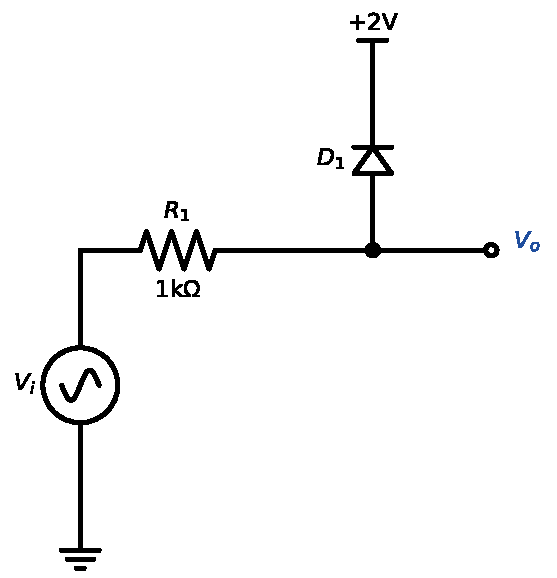
\includegraphics[width=0.9\linewidth,height=5cm,keepaspectratio]{p04_circuit}\end{center}
\solstep{1}{Model and method}Use the constant-voltage-drop model (tool T1): an OFF diode is an open circuit and needs $V_D<0.7$\,V; an ON diode is a $0.7$\,V source and needs $I_D>0$. With 1 diode there are $2$ ON/OFF combinations. For each one the circuit is linear: solve it with $V_i$ kept as a symbol, then check its assumptions --- each check is a condition on $V_i$ (tool T2).
\solstep{2}{Assume $D_{1}$ OFF}Replace $D_{1}$ OFF: an open circuit.

Equations (KCL at every node that is not an op-amp output, plus the diode voltages):\begin{align*}
&\text{KCL at }V_{o}: && \frac{V_{o} - V_i}{R_{1}} = 0
\end{align*}


Solving these linear equations (substitute one into the other, as in Lecture 2) gives, with $V_i$ kept as a symbol:\begin{align*}
V_{o} &= V_i \\
V_{D_{1}} = V_{o} - 2 &= V_i - 2
\end{align*}


Check the assumptions: $V_{D_{1}} < 0.7$ $\Rightarrow$ $V_i < 2.7$\,V. So this state holds for $\boxed{V_i < 2.7}$, where $V_o = V_i$.
\solstep{3}{Assume $D_{1}$ ON}Replace $D_{1}$ ON: a $0.7$\,V source ($V_{o} - 2 = 0.7$) carrying an unknown current $I_{D_{1}}$ from anode to cathode.

Equations (KCL at every node that is not an op-amp output, plus the diode voltages):\begin{align*}
&\text{KCL at }V_{o}: && \frac{V_{o} - V_i}{R_{1}} + I_{D_{1}} = 0 \\
&\text{D1 ON}: && V_{o} - 2 = 0.7
\end{align*}


Solving these linear equations (substitute one into the other, as in Lecture 2) gives, with $V_i$ kept as a symbol:\begin{align*}
V_{o} &= 2.7 \\
I_{D_{1}} &= V_i - 2.7\ \mathrm{mA}
\end{align*}


Check the assumptions: $I_{D_{1}} > 0$ $\Rightarrow$ $V_i > 2.7$\,V. So this state holds for $\boxed{V_i > 2.7}$, where $V_o = 2.7$.
\solstep{4}{Assemble and sketch}Put the valid states together:\[
V_o = \begin{cases} V_i & V_i < 2.7 \\ 2.7 & V_i > 2.7 \end{cases}
\]
Check: the pieces must meet at each breakpoint --- at $V_i=2.7$\,V both pieces give $V_o=2.7$\,V. \checkmark\begin{center}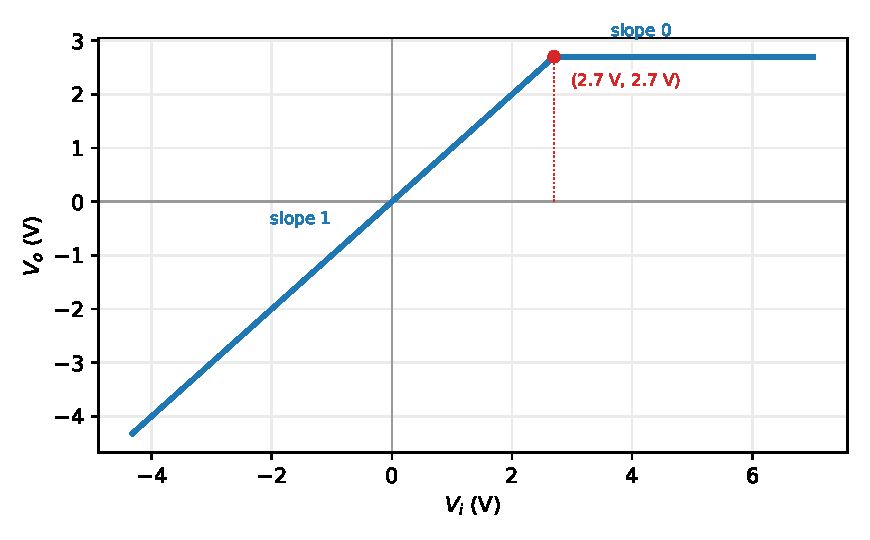
\includegraphics[width=0.62\linewidth,height=6cm,keepaspectratio]{p04_transfer}\end{center}
For $V_i(t) = 5\sin(2\pi\cdot 1000\,t)$ simply pass every instant of $V_i(t)$ through the characteristic above (each piece is a straight line, so each part of the sinusoid is scaled and shifted):\begin{center}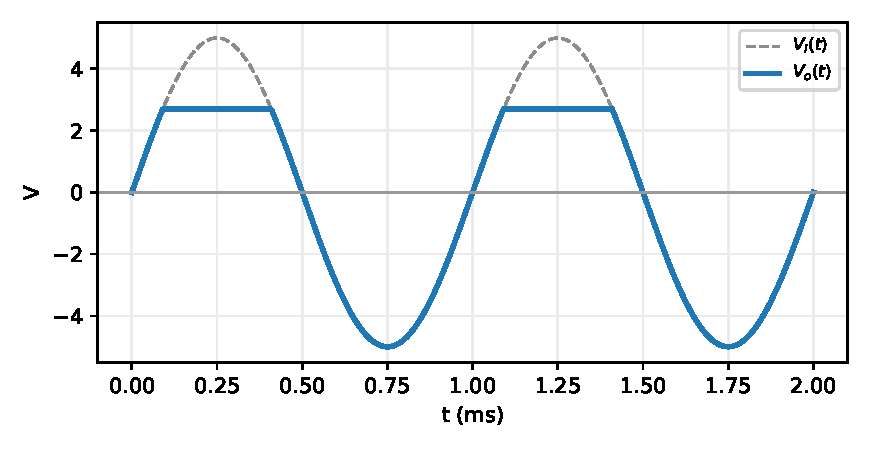
\includegraphics[width=0.62\linewidth,height=5cm,keepaspectratio]{p04_time}\end{center}

\begin{ansbox}
$V_o = \begin{cases} V_i & V_i < 2.7 \\ 2.7 & V_i > 2.7 \end{cases}$
\end{ansbox}

\newpage
\subsection*{Solution 3A.5 \hfill Easy}
\begin{center}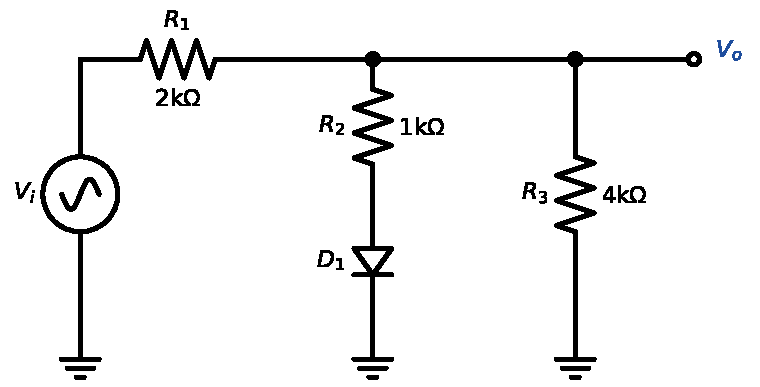
\includegraphics[width=0.9\linewidth,height=5cm,keepaspectratio]{p05_circuit}\end{center}
\solstep{1}{Model and method}Use the constant-voltage-drop model (tool T1): an OFF diode is an open circuit and needs $V_D<0.7$\,V; an ON diode is a $0.7$\,V source and needs $I_D>0$. With 1 diode there are $2$ ON/OFF combinations. For each one the circuit is linear: solve it with $V_i$ kept as a symbol, then check its assumptions --- each check is a condition on $V_i$ (tool T2). Node names used below: $V_{a}$ = node joining $D_{1}, R_{2}$.
\solstep{2}{Assume $D_{1}$ OFF}Replace $D_{1}$ OFF: an open circuit.

Equations (KCL at every node that is not an op-amp output, plus the diode voltages):\begin{align*}
&\text{KCL at }V_{a}: && \frac{V_{a} - V_{o}}{R_{2}} = 0 \\
&\text{KCL at }V_{o}: && \frac{V_{o} - V_i}{R_{1}} + \frac{V_{o} - V_{a}}{R_{2}} + \frac{V_{o}}{R_{3}} = 0
\end{align*}


Solving these linear equations (substitute one into the other, as in Lecture 2) gives, with $V_i$ kept as a symbol:\begin{align*}
V_{o} &= 0.6667V_i \\
V_{D_{1}} = V_{a} - 0 &= 0.6667V_i
\end{align*}


Check the assumptions: $V_{D_{1}} < 0.7$ $\Rightarrow$ $V_i < 1.05$\,V. So this state holds for $\boxed{V_i < 1.05}$, where $V_o = 0.6667V_i$.
\solstep{3}{Assume $D_{1}$ ON}Replace $D_{1}$ ON: a $0.7$\,V source ($V_{a} - 0 = 0.7$) carrying an unknown current $I_{D_{1}}$ from anode to cathode.

Equations (KCL at every node that is not an op-amp output, plus the diode voltages):\begin{align*}
&\text{KCL at }V_{a}: && \frac{V_{a} - V_{o}}{R_{2}} + I_{D_{1}} = 0 \\
&\text{KCL at }V_{o}: && \frac{V_{o} - V_i}{R_{1}} + \frac{V_{o} - V_{a}}{R_{2}} + \frac{V_{o}}{R_{3}} = 0 \\
&\text{D1 ON}: && V_{a} - 0 = 0.7
\end{align*}


Solving these linear equations (substitute one into the other, as in Lecture 2) gives, with $V_i$ kept as a symbol:\begin{align*}
V_{o} &= 0.2857V_i + 0.4 \\
I_{D_{1}} &= 0.2857V_i - 0.3\ \mathrm{mA}
\end{align*}


Check the assumptions: $I_{D_{1}} > 0$ $\Rightarrow$ $V_i > 1.05$\,V. So this state holds for $\boxed{V_i > 1.05}$, where $V_o = 0.2857V_i + 0.4$.
\solstep{4}{Assemble and sketch}Put the valid states together:\[
V_o = \begin{cases} 0.6667V_i & V_i < 1.05 \\ 0.2857V_i + 0.4 & V_i > 1.05 \end{cases}
\]
Check: the pieces must meet at each breakpoint --- at $V_i=1.05$\,V both pieces give $V_o=0.7$\,V. \checkmark\begin{center}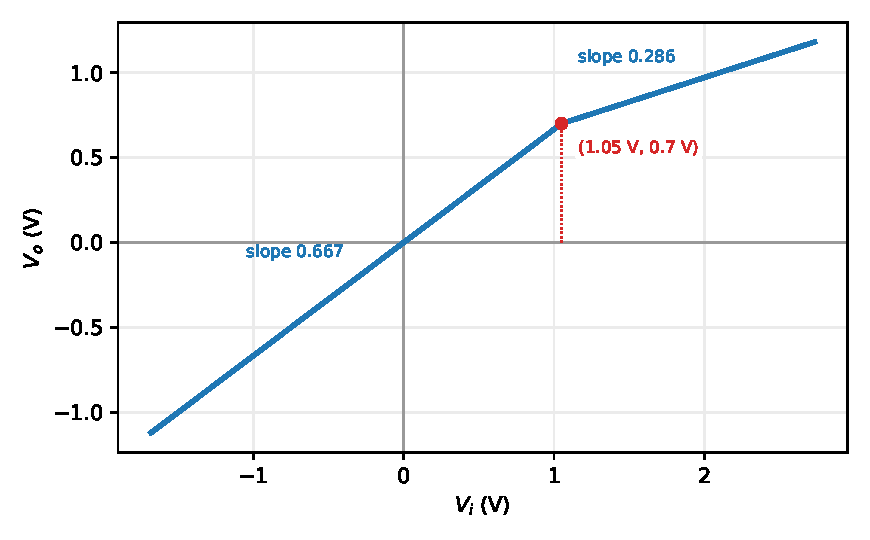
\includegraphics[width=0.62\linewidth,height=6cm,keepaspectratio]{p05_transfer}\end{center}

\begin{ansbox}
$V_o = \begin{cases} 0.6667V_i & V_i < 1.05 \\ 0.2857V_i + 0.4 & V_i > 1.05 \end{cases}$
\end{ansbox}

\newpage
\subsection*{Solution 3A.6 \hfill Easy}
\begin{center}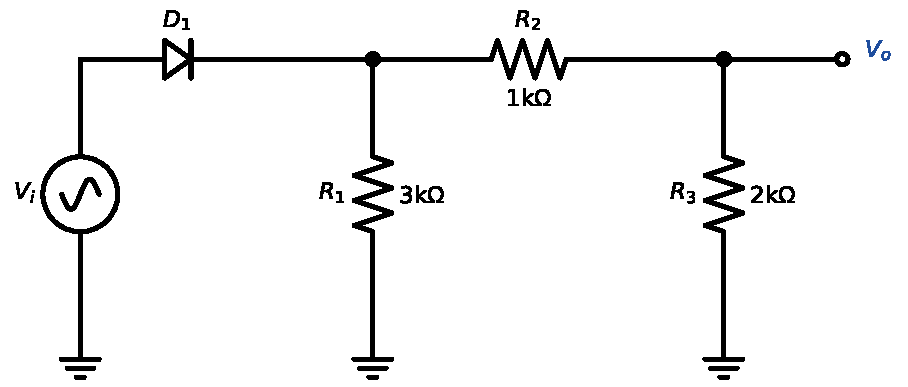
\includegraphics[width=0.9\linewidth,height=5cm,keepaspectratio]{p06_circuit}\end{center}
\solstep{1}{Model and method}Use the ideal-diode model (tool T1): an OFF diode is an open circuit and needs $V_D<0$; an ON diode is a short ($V_D=0$) and needs $I_D>0$. With 1 diode there are $2$ ON/OFF combinations. For each one the circuit is linear: solve it with $V_i$ kept as a symbol, then check its assumptions --- each check is a condition on $V_i$ (tool T2). Node names used below: $V_{1}$ = node joining $D_{1}, R_{1}, R_{2}$.
\solstep{2}{Assume $D_{1}$ OFF}Replace $D_{1}$ OFF: an open circuit.

Equations (KCL at every node that is not an op-amp output, plus the diode voltages):\begin{align*}
&\text{KCL at }V_{1}: && \frac{V_{1}}{R_{1}} + \frac{V_{1} - V_{o}}{R_{2}} = 0 \\
&\text{KCL at }V_{o}: && \frac{V_{o} - V_{1}}{R_{2}} + \frac{V_{o}}{R_{3}} = 0
\end{align*}


Solving these linear equations (substitute one into the other, as in Lecture 2) gives, with $V_i$ kept as a symbol:\begin{align*}
V_{o} &= 0 \\
V_{D_{1}} = V_i - V_{1} &= V_i
\end{align*}


Check the assumptions: $V_{D_{1}} < 0$ $\Rightarrow$ $V_i < 0$\,V. So this state holds for $\boxed{V_i < 0}$, where $V_o = 0$.
\solstep{3}{Assume $D_{1}$ ON}Replace $D_{1}$ ON: a $0$\,V source ($V_i - V_{1} = 0$) carrying an unknown current $I_{D_{1}}$ from anode to cathode.

Equations (KCL at every node that is not an op-amp output, plus the diode voltages):\begin{align*}
&\text{KCL at }V_{1}: && \frac{V_{1}}{R_{1}} + \frac{V_{1} - V_{o}}{R_{2}} - I_{D_{1}} = 0 \\
&\text{KCL at }V_{o}: && \frac{V_{o} - V_{1}}{R_{2}} + \frac{V_{o}}{R_{3}} = 0 \\
&\text{D1 ON}: && V_i - V_{1} = 0
\end{align*}


Solving these linear equations (substitute one into the other, as in Lecture 2) gives, with $V_i$ kept as a symbol:\begin{align*}
V_{o} &= 0.6667V_i \\
I_{D_{1}} &= 0.6667V_i\ \mathrm{mA}
\end{align*}


Check the assumptions: $I_{D_{1}} > 0$ $\Rightarrow$ $V_i > 0$\,V. So this state holds for $\boxed{V_i > 0}$, where $V_o = 0.6667V_i$.
\solstep{4}{Assemble and sketch}Put the valid states together:\[
V_o = \begin{cases} 0 & V_i < 0 \\ 0.6667V_i & V_i > 0 \end{cases}
\]
Check: the pieces must meet at each breakpoint --- at $V_i=0$\,V both pieces give $V_o=0$\,V. \checkmark\begin{center}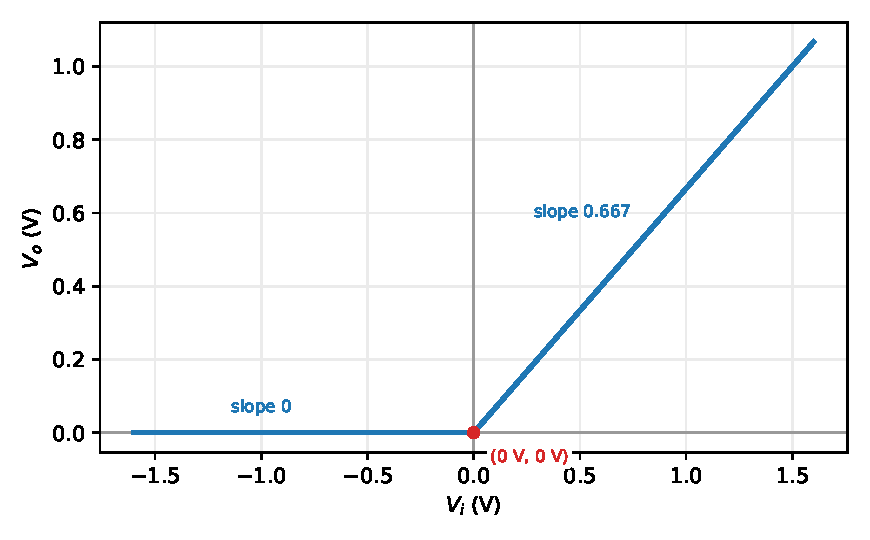
\includegraphics[width=0.62\linewidth,height=6cm,keepaspectratio]{p06_transfer}\end{center}

\begin{ansbox}
$V_o = \begin{cases} 0 & V_i < 0 \\ 0.6667V_i & V_i > 0 \end{cases}$
\end{ansbox}

\newpage
\subsection*{Solution 3A.7 \hfill Medium}
\begin{center}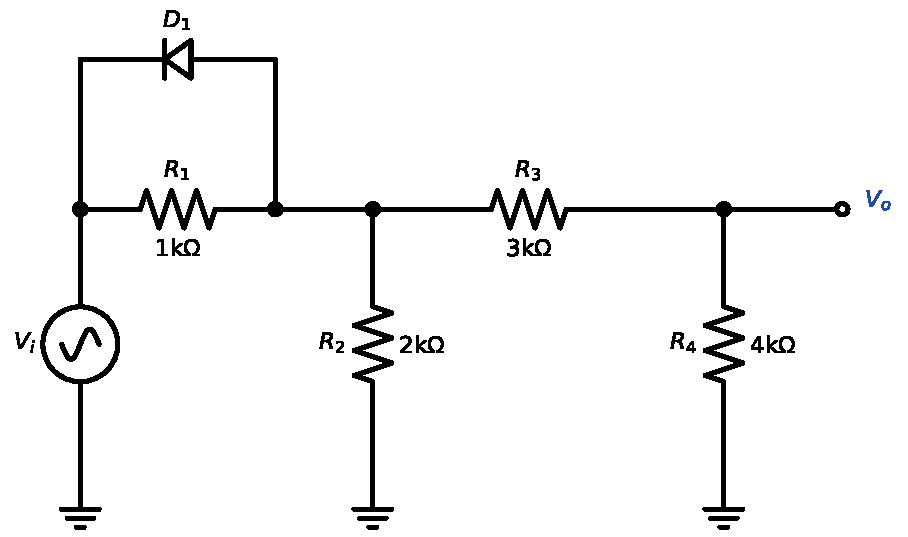
\includegraphics[width=0.9\linewidth,height=5cm,keepaspectratio]{p07_circuit}\end{center}
\solstep{1}{Model and method}Use the constant-voltage-drop model (tool T1): an OFF diode is an open circuit and needs $V_D<0.7$\,V; an ON diode is a $0.7$\,V source and needs $I_D>0$. With 1 diode there are $2$ ON/OFF combinations. For each one the circuit is linear: solve it with $V_i$ kept as a symbol, then check its assumptions --- each check is a condition on $V_i$ (tool T2). Node names used below: $V_{1}$ = node joining $D_{1}, R_{1}, R_{2}, R_{3}$.
\solstep{2}{Assume $D_{1}$ ON}Replace $D_{1}$ ON: a $0.7$\,V source ($V_{1} - V_i = 0.7$) carrying an unknown current $I_{D_{1}}$ from anode to cathode.

Equations (KCL at every node that is not an op-amp output, plus the diode voltages):\begin{align*}
&\text{KCL at }V_{1}: && \frac{V_{1} - V_i}{R_{1}} + \frac{V_{1}}{R_{2}} + \frac{V_{1} - V_{o}}{R_{3}} + I_{D_{1}} = 0 \\
&\text{KCL at }V_{o}: && \frac{V_{o} - V_{1}}{R_{3}} + \frac{V_{o}}{R_{4}} = 0 \\
&\text{D1 ON}: && V_{1} - V_i = 0.7
\end{align*}


Solving these linear equations (substitute one into the other, as in Lecture 2) gives, with $V_i$ kept as a symbol:\begin{align*}
V_{o} &= 0.5714V_i + 0.4 \\
I_{D_{1}} &= -0.6429V_i - 1.15\ \mathrm{mA}
\end{align*}


Check the assumptions: $I_{D_{1}} > 0$ $\Rightarrow$ $V_i < -1.789$\,V. So this state holds for $\boxed{V_i < -1.789}$, where $V_o = 0.5714V_i + 0.4$.
\solstep{3}{Assume $D_{1}$ OFF}Replace $D_{1}$ OFF: an open circuit.

Equations (KCL at every node that is not an op-amp output, plus the diode voltages):\begin{align*}
&\text{KCL at }V_{1}: && \frac{V_{1} - V_i}{R_{1}} + \frac{V_{1}}{R_{2}} + \frac{V_{1} - V_{o}}{R_{3}} = 0 \\
&\text{KCL at }V_{o}: && \frac{V_{o} - V_{1}}{R_{3}} + \frac{V_{o}}{R_{4}} = 0
\end{align*}


Solving these linear equations (substitute one into the other, as in Lecture 2) gives, with $V_i$ kept as a symbol:\begin{align*}
V_{o} &= 0.3478V_i \\
V_{D_{1}} = V_{1} - V_i &= -0.3913V_i
\end{align*}


Check the assumptions: $V_{D_{1}} < 0.7$ $\Rightarrow$ $V_i > -1.789$\,V. So this state holds for $\boxed{V_i > -1.789}$, where $V_o = 0.3478V_i$.
\solstep{4}{Assemble and sketch}Put the valid states together:\[
V_o = \begin{cases} 0.5714V_i + 0.4 & V_i < -1.789 \\ 0.3478V_i & V_i > -1.789 \end{cases}
\]
Check: the pieces must meet at each breakpoint --- at $V_i=-1.789$\,V both pieces give $V_o=-0.6222$\,V. \checkmark\begin{center}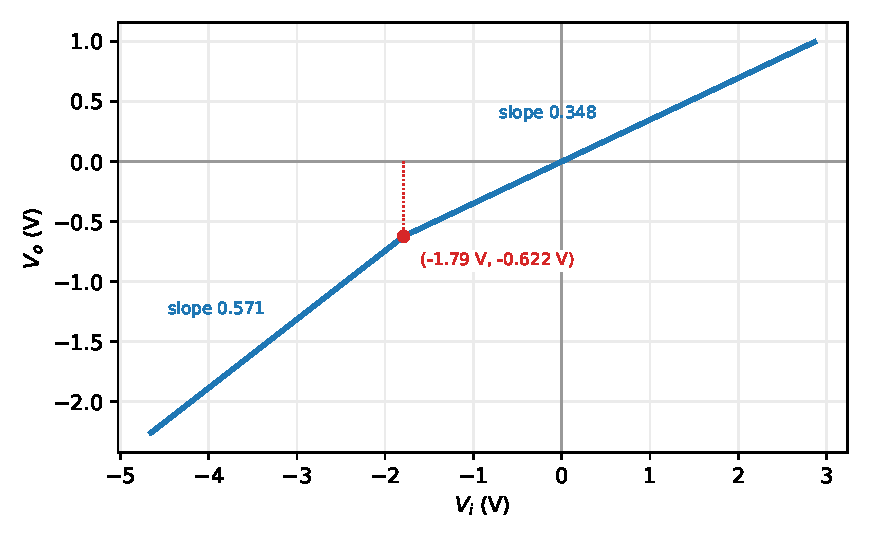
\includegraphics[width=0.62\linewidth,height=6cm,keepaspectratio]{p07_transfer}\end{center}

\begin{ansbox}
$V_o = \begin{cases} 0.5714V_i + 0.4 & V_i < -1.789 \\ 0.3478V_i & V_i > -1.789 \end{cases}$
\end{ansbox}

\newpage
\subsection*{Solution 3A.8 \hfill Medium}
\begin{center}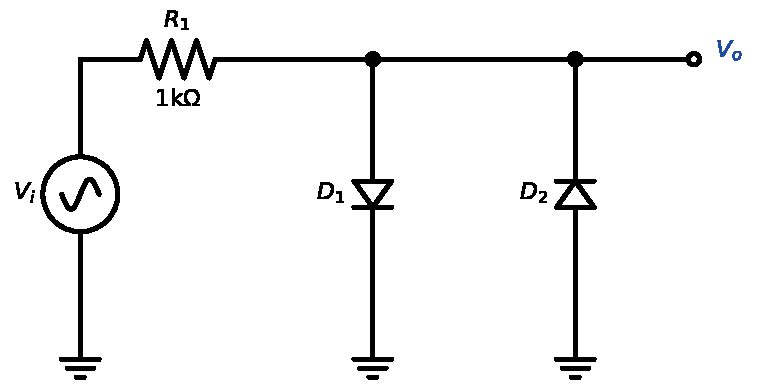
\includegraphics[width=0.9\linewidth,height=5cm,keepaspectratio]{p08_circuit}\end{center}
\solstep{1}{Model and method}Use the constant-voltage-drop model (tool T1): an OFF diode is an open circuit and needs $V_D<0.7$\,V; an ON diode is a $0.7$\,V source and needs $I_D>0$. With 2 diodes there are $4$ ON/OFF combinations. For each one the circuit is linear: solve it with $V_i$ kept as a symbol, then check its assumptions --- each check is a condition on $V_i$ (tool T2).
\solstep{2}{Assume $D_{1}$ OFF, $D_{2}$ ON}Replace $D_{1}$ OFF: an open circuit; $D_{2}$ ON: a $0.7$\,V source ($0 - V_{o} = 0.7$) carrying an unknown current $I_{D_{2}}$ from anode to cathode.

Equations (KCL at every node that is not an op-amp output, plus the diode voltages):\begin{align*}
&\text{KCL at }V_{o}: && \frac{V_{o} - V_i}{R_{1}} - I_{D_{2}} = 0 \\
&\text{D2 ON}: && 0 - V_{o} = 0.7
\end{align*}


Solving these linear equations (substitute one into the other, as in Lecture 2) gives, with $V_i$ kept as a symbol:\begin{align*}
V_{o} &= -0.7 \\
V_{D_{1}} = V_{o} - 0 &= -0.7 \\
I_{D_{2}} &= -V_i - 0.7\ \mathrm{mA}
\end{align*}


Check the assumptions: $V_{D_{1}} < 0.7$ $\Rightarrow$ true for every $V_i$; $I_{D_{2}} > 0$ $\Rightarrow$ $V_i < -0.7$\,V. So this state holds for $\boxed{V_i < -0.7}$, where $V_o = -0.7$.
\solstep{3}{Assume $D_{1}$ OFF, $D_{2}$ OFF}Replace $D_{1}$ OFF: an open circuit; $D_{2}$ OFF: an open circuit.

Equations (KCL at every node that is not an op-amp output, plus the diode voltages):\begin{align*}
&\text{KCL at }V_{o}: && \frac{V_{o} - V_i}{R_{1}} = 0
\end{align*}


Solving these linear equations (substitute one into the other, as in Lecture 2) gives, with $V_i$ kept as a symbol:\begin{align*}
V_{o} &= V_i \\
V_{D_{1}} = V_{o} - 0 &= V_i \\
V_{D_{2}} = 0 - V_{o} &= -V_i
\end{align*}


Check the assumptions: $V_{D_{1}} < 0.7$ $\Rightarrow$ $V_i < 0.7$\,V; $V_{D_{2}} < 0.7$ $\Rightarrow$ $V_i > -0.7$\,V. So this state holds for $\boxed{-0.7 < V_i < 0.7}$, where $V_o = V_i$.
\solstep{4}{Assume $D_{1}$ ON, $D_{2}$ OFF}Replace $D_{1}$ ON: a $0.7$\,V source ($V_{o} - 0 = 0.7$) carrying an unknown current $I_{D_{1}}$ from anode to cathode; $D_{2}$ OFF: an open circuit.

Equations (KCL at every node that is not an op-amp output, plus the diode voltages):\begin{align*}
&\text{KCL at }V_{o}: && \frac{V_{o} - V_i}{R_{1}} + I_{D_{1}} = 0 \\
&\text{D1 ON}: && V_{o} - 0 = 0.7
\end{align*}


Solving these linear equations (substitute one into the other, as in Lecture 2) gives, with $V_i$ kept as a symbol:\begin{align*}
V_{o} &= 0.7 \\
I_{D_{1}} &= V_i - 0.7\ \mathrm{mA} \\
V_{D_{2}} = 0 - V_{o} &= -0.7
\end{align*}


Check the assumptions: $I_{D_{1}} > 0$ $\Rightarrow$ $V_i > 0.7$\,V; $V_{D_{2}} < 0.7$ $\Rightarrow$ true for every $V_i$. So this state holds for $\boxed{V_i > 0.7}$, where $V_o = 0.7$.
\solstep{5}{The other combinations}\begin{itemize}[leftmargin=*,itemsep=2pt]
\item $D_{1}$ ON, $D_{2}$ ON: the ON diodes would have to hold the same node at two different voltages at once, which no circuit can do --- these cannot all hold, so this state never occurs.
\end{itemize}

\solstep{6}{Assemble and sketch}Put the valid states together:\[
V_o = \begin{cases} -0.7 & V_i < -0.7 \\ V_i & -0.7 < V_i < 0.7 \\ 0.7 & V_i > 0.7 \end{cases}
\]
Check: the pieces must meet at each breakpoint --- at $V_i=-0.7$\,V both pieces give $V_o=-0.7$\,V; at $V_i=0.7$\,V both pieces give $V_o=0.7$\,V. \checkmark\begin{center}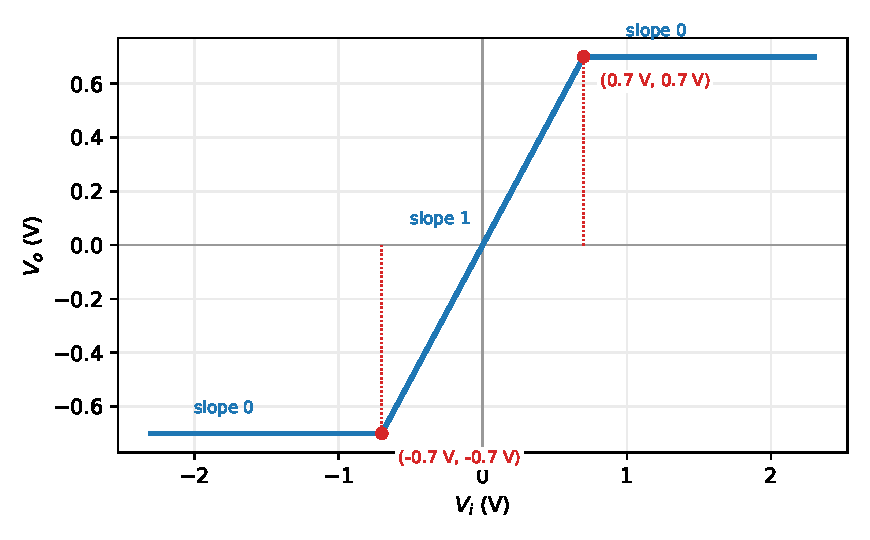
\includegraphics[width=0.62\linewidth,height=6cm,keepaspectratio]{p08_transfer}\end{center}
For $V_i(t) = 2\sin(2\pi\cdot 1000\,t)$ simply pass every instant of $V_i(t)$ through the characteristic above (each piece is a straight line, so each part of the sinusoid is scaled and shifted):\begin{center}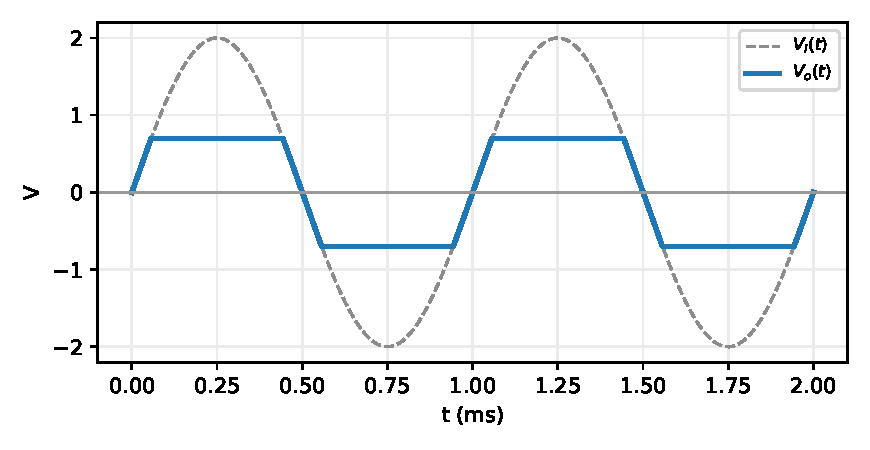
\includegraphics[width=0.62\linewidth,height=5cm,keepaspectratio]{p08_time}\end{center}

\begin{ansbox}
$V_o = \begin{cases} -0.7 & V_i < -0.7 \\ V_i & -0.7 < V_i < 0.7 \\ 0.7 & V_i > 0.7 \end{cases}$
\end{ansbox}

\newpage
\subsection*{Solution 3A.9 \hfill Medium}
\begin{center}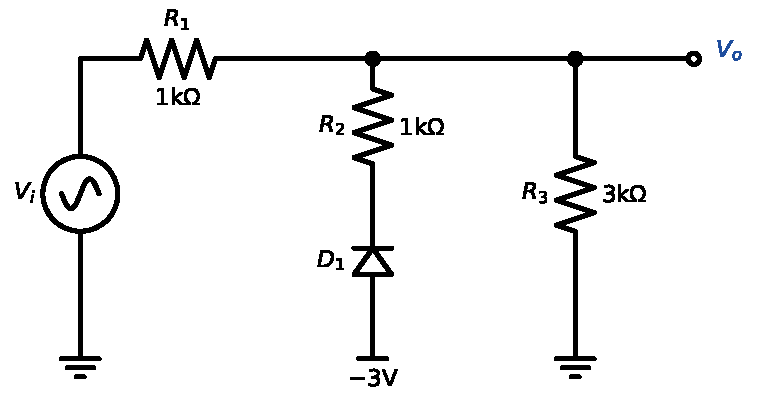
\includegraphics[width=0.9\linewidth,height=5cm,keepaspectratio]{p09_circuit}\end{center}
\solstep{1}{Model and method}Use the constant-voltage-drop model (tool T1): an OFF diode is an open circuit and needs $V_D<0.7$\,V; an ON diode is a $0.7$\,V source and needs $I_D>0$. With 1 diode there are $2$ ON/OFF combinations. For each one the circuit is linear: solve it with $V_i$ kept as a symbol, then check its assumptions --- each check is a condition on $V_i$ (tool T2). Node names used below: $V_{a}$ = node joining $D_{1}, R_{2}$.
\solstep{2}{Assume $D_{1}$ ON}Replace $D_{1}$ ON: a $0.7$\,V source ($-3 - V_{a} = 0.7$) carrying an unknown current $I_{D_{1}}$ from anode to cathode.

Equations (KCL at every node that is not an op-amp output, plus the diode voltages):\begin{align*}
&\text{KCL at }V_{a}: && \frac{V_{a} - V_{o}}{R_{2}} - I_{D_{1}} = 0 \\
&\text{KCL at }V_{o}: && \frac{V_{o} - V_i}{R_{1}} + \frac{V_{o} - V_{a}}{R_{2}} + \frac{V_{o}}{R_{3}} = 0 \\
&\text{D1 ON}: && -3 - V_{a} = 0.7
\end{align*}


Solving these linear equations (substitute one into the other, as in Lecture 2) gives, with $V_i$ kept as a symbol:\begin{align*}
V_{o} &= 0.4286V_i - 1.586 \\
I_{D_{1}} &= -0.4286V_i - 2.114\ \mathrm{mA}
\end{align*}


Check the assumptions: $I_{D_{1}} > 0$ $\Rightarrow$ $V_i < -4.933$\,V. So this state holds for $\boxed{V_i < -4.933}$, where $V_o = 0.4286V_i - 1.586$.
\solstep{3}{Assume $D_{1}$ OFF}Replace $D_{1}$ OFF: an open circuit.

Equations (KCL at every node that is not an op-amp output, plus the diode voltages):\begin{align*}
&\text{KCL at }V_{a}: && \frac{V_{a} - V_{o}}{R_{2}} = 0 \\
&\text{KCL at }V_{o}: && \frac{V_{o} - V_i}{R_{1}} + \frac{V_{o} - V_{a}}{R_{2}} + \frac{V_{o}}{R_{3}} = 0
\end{align*}


Solving these linear equations (substitute one into the other, as in Lecture 2) gives, with $V_i$ kept as a symbol:\begin{align*}
V_{o} &= 0.75V_i \\
V_{D_{1}} = -3 - V_{a} &= -0.75V_i - 3
\end{align*}


Check the assumptions: $V_{D_{1}} < 0.7$ $\Rightarrow$ $V_i > -4.933$\,V. So this state holds for $\boxed{V_i > -4.933}$, where $V_o = 0.75V_i$.
\solstep{4}{Assemble and sketch}Put the valid states together:\[
V_o = \begin{cases} 0.4286V_i - 1.586 & V_i < -4.933 \\ 0.75V_i & V_i > -4.933 \end{cases}
\]
Check: the pieces must meet at each breakpoint --- at $V_i=-4.933$\,V both pieces give $V_o=-3.7$\,V. \checkmark\begin{center}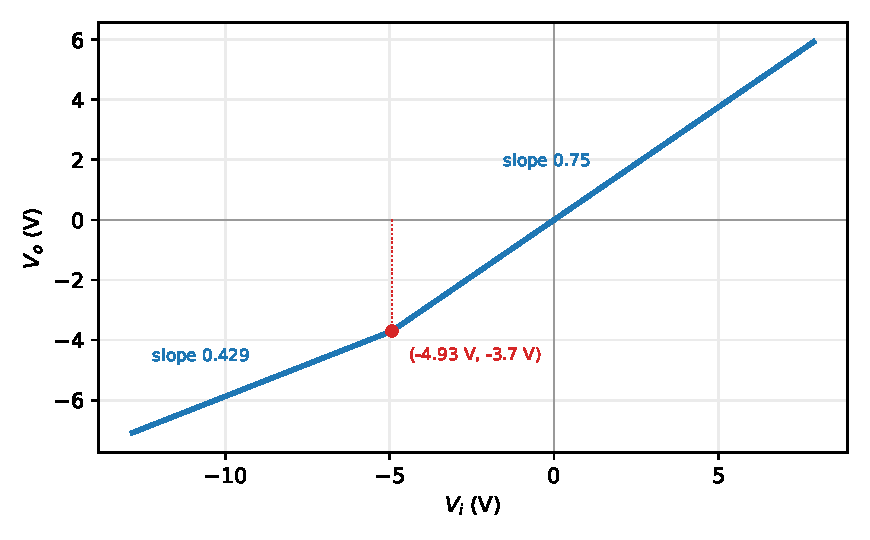
\includegraphics[width=0.62\linewidth,height=6cm,keepaspectratio]{p09_transfer}\end{center}

\begin{ansbox}
$V_o = \begin{cases} 0.4286V_i - 1.586 & V_i < -4.933 \\ 0.75V_i & V_i > -4.933 \end{cases}$
\end{ansbox}

\newpage
\subsection*{Solution 3A.10 \hfill Medium}
\begin{center}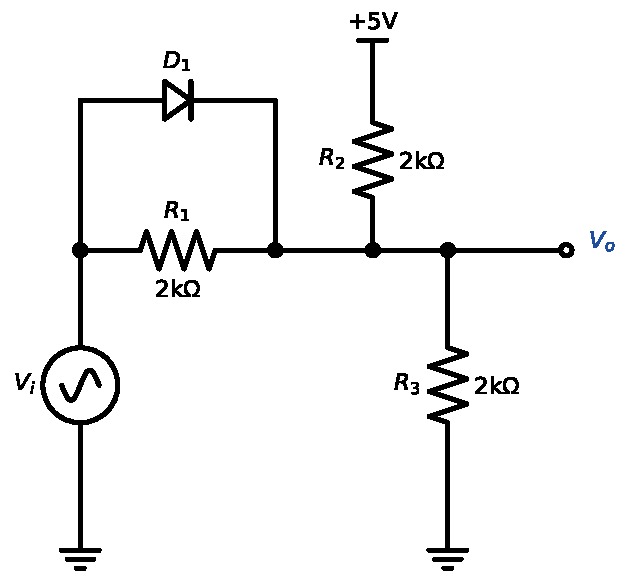
\includegraphics[width=0.9\linewidth,height=5cm,keepaspectratio]{p10_circuit}\end{center}
\solstep{1}{Model and method}Use the constant-voltage-drop model (tool T1): an OFF diode is an open circuit and needs $V_D<0.7$\,V; an ON diode is a $0.7$\,V source and needs $I_D>0$. With 1 diode there are $2$ ON/OFF combinations. For each one the circuit is linear: solve it with $V_i$ kept as a symbol, then check its assumptions --- each check is a condition on $V_i$ (tool T2).
\solstep{2}{Assume $D_{1}$ OFF}Replace $D_{1}$ OFF: an open circuit.

Equations (KCL at every node that is not an op-amp output, plus the diode voltages):\begin{align*}
&\text{KCL at }V_{o}: && \frac{V_{o} - V_i}{R_{1}} + \frac{V_{o} - 5}{R_{2}} + \frac{V_{o}}{R_{3}} = 0
\end{align*}


Solving these linear equations (substitute one into the other, as in Lecture 2) gives, with $V_i$ kept as a symbol:\begin{align*}
V_{o} &= 0.3333V_i + 1.667 \\
V_{D_{1}} = V_i - V_{o} &= 0.6667V_i - 1.667
\end{align*}


Check the assumptions: $V_{D_{1}} < 0.7$ $\Rightarrow$ $V_i < 3.55$\,V. So this state holds for $\boxed{V_i < 3.55}$, where $V_o = 0.3333V_i + 1.667$.
\solstep{3}{Assume $D_{1}$ ON}Replace $D_{1}$ ON: a $0.7$\,V source ($V_i - V_{o} = 0.7$) carrying an unknown current $I_{D_{1}}$ from anode to cathode.

Equations (KCL at every node that is not an op-amp output, plus the diode voltages):\begin{align*}
&\text{KCL at }V_{o}: && \frac{V_{o} - V_i}{R_{1}} + \frac{V_{o} - 5}{R_{2}} + \frac{V_{o}}{R_{3}} - I_{D_{1}} = 0 \\
&\text{D1 ON}: && V_i - V_{o} = 0.7
\end{align*}


Solving these linear equations (substitute one into the other, as in Lecture 2) gives, with $V_i$ kept as a symbol:\begin{align*}
V_{o} &= V_i - 0.7 \\
I_{D_{1}} &= V_i - 3.55\ \mathrm{mA}
\end{align*}


Check the assumptions: $I_{D_{1}} > 0$ $\Rightarrow$ $V_i > 3.55$\,V. So this state holds for $\boxed{V_i > 3.55}$, where $V_o = V_i - 0.7$.
\solstep{4}{Assemble and sketch}Put the valid states together:\[
V_o = \begin{cases} 0.3333V_i + 1.667 & V_i < 3.55 \\ V_i - 0.7 & V_i > 3.55 \end{cases}
\]
Check: the pieces must meet at each breakpoint --- at $V_i=3.55$\,V both pieces give $V_o=2.85$\,V. \checkmark\begin{center}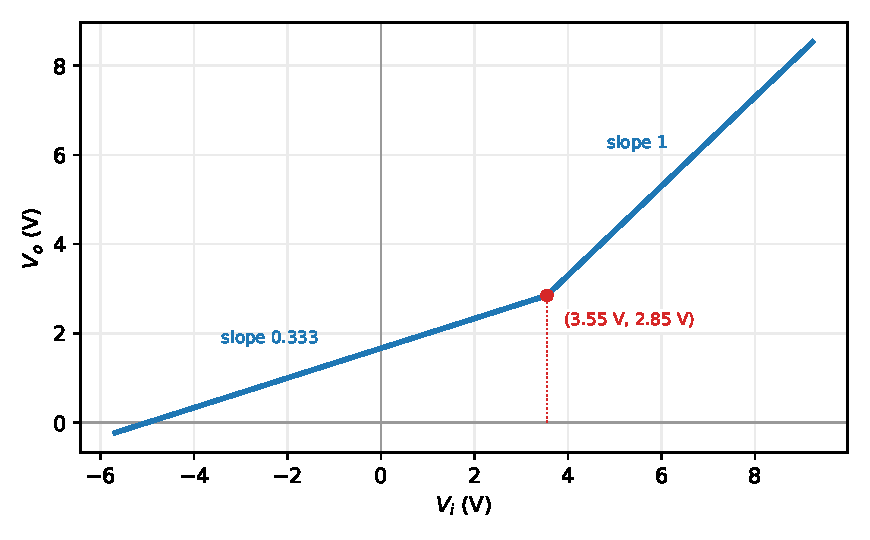
\includegraphics[width=0.62\linewidth,height=6cm,keepaspectratio]{p10_transfer}\end{center}

\begin{ansbox}
$V_o = \begin{cases} 0.3333V_i + 1.667 & V_i < 3.55 \\ V_i - 0.7 & V_i > 3.55 \end{cases}$
\end{ansbox}

\newpage
\subsection*{Solution 3A.11 \hfill Medium}
\begin{center}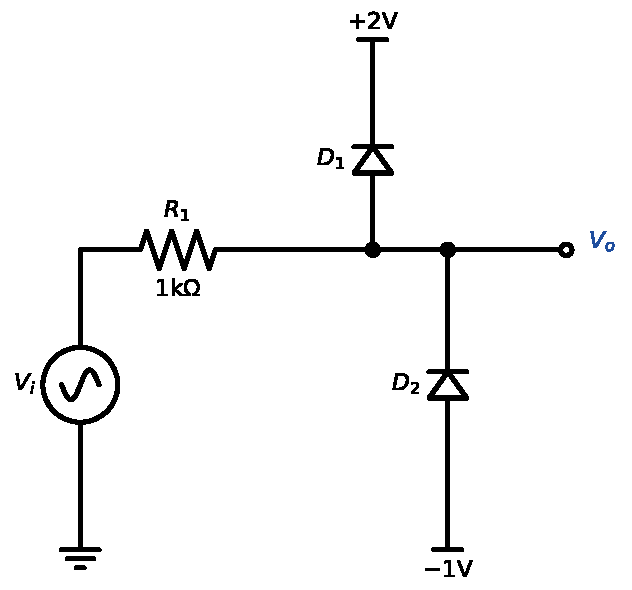
\includegraphics[width=0.9\linewidth,height=5cm,keepaspectratio]{p11_circuit}\end{center}
\solstep{1}{Model and method}Use the ideal-diode model (tool T1): an OFF diode is an open circuit and needs $V_D<0$; an ON diode is a short ($V_D=0$) and needs $I_D>0$. With 2 diodes there are $4$ ON/OFF combinations. For each one the circuit is linear: solve it with $V_i$ kept as a symbol, then check its assumptions --- each check is a condition on $V_i$ (tool T2).
\solstep{2}{Assume $D_{1}$ OFF, $D_{2}$ ON}Replace $D_{1}$ OFF: an open circuit; $D_{2}$ ON: a $0$\,V source ($-1 - V_{o} = 0$) carrying an unknown current $I_{D_{2}}$ from anode to cathode.

Equations (KCL at every node that is not an op-amp output, plus the diode voltages):\begin{align*}
&\text{KCL at }V_{o}: && \frac{V_{o} - V_i}{R_{1}} - I_{D_{2}} = 0 \\
&\text{D2 ON}: && -1 - V_{o} = 0
\end{align*}


Solving these linear equations (substitute one into the other, as in Lecture 2) gives, with $V_i$ kept as a symbol:\begin{align*}
V_{o} &= -1 \\
V_{D_{1}} = V_{o} - 2 &= -3 \\
I_{D_{2}} &= -V_i - 1\ \mathrm{mA}
\end{align*}


Check the assumptions: $V_{D_{1}} < 0$ $\Rightarrow$ true for every $V_i$; $I_{D_{2}} > 0$ $\Rightarrow$ $V_i < -1$\,V. So this state holds for $\boxed{V_i < -1}$, where $V_o = -1$.
\solstep{3}{Assume $D_{1}$ OFF, $D_{2}$ OFF}Replace $D_{1}$ OFF: an open circuit; $D_{2}$ OFF: an open circuit.

Equations (KCL at every node that is not an op-amp output, plus the diode voltages):\begin{align*}
&\text{KCL at }V_{o}: && \frac{V_{o} - V_i}{R_{1}} = 0
\end{align*}


Solving these linear equations (substitute one into the other, as in Lecture 2) gives, with $V_i$ kept as a symbol:\begin{align*}
V_{o} &= V_i \\
V_{D_{1}} = V_{o} - 2 &= V_i - 2 \\
V_{D_{2}} = -1 - V_{o} &= -V_i - 1
\end{align*}


Check the assumptions: $V_{D_{1}} < 0$ $\Rightarrow$ $V_i < 2$\,V; $V_{D_{2}} < 0$ $\Rightarrow$ $V_i > -1$\,V. So this state holds for $\boxed{-1 < V_i < 2}$, where $V_o = V_i$.
\solstep{4}{Assume $D_{1}$ ON, $D_{2}$ OFF}Replace $D_{1}$ ON: a $0$\,V source ($V_{o} - 2 = 0$) carrying an unknown current $I_{D_{1}}$ from anode to cathode; $D_{2}$ OFF: an open circuit.

Equations (KCL at every node that is not an op-amp output, plus the diode voltages):\begin{align*}
&\text{KCL at }V_{o}: && \frac{V_{o} - V_i}{R_{1}} + I_{D_{1}} = 0 \\
&\text{D1 ON}: && V_{o} - 2 = 0
\end{align*}


Solving these linear equations (substitute one into the other, as in Lecture 2) gives, with $V_i$ kept as a symbol:\begin{align*}
V_{o} &= 2 \\
I_{D_{1}} &= V_i - 2\ \mathrm{mA} \\
V_{D_{2}} = -1 - V_{o} &= -3
\end{align*}


Check the assumptions: $I_{D_{1}} > 0$ $\Rightarrow$ $V_i > 2$\,V; $V_{D_{2}} < 0$ $\Rightarrow$ true for every $V_i$. So this state holds for $\boxed{V_i > 2}$, where $V_o = 2$.
\solstep{5}{The other combinations}\begin{itemize}[leftmargin=*,itemsep=2pt]
\item $D_{1}$ ON, $D_{2}$ ON: the ON diodes would have to hold the same node at two different voltages at once, which no circuit can do --- these cannot all hold, so this state never occurs.
\end{itemize}

\solstep{6}{Assemble and sketch}Put the valid states together:\[
V_o = \begin{cases} -1 & V_i < -1 \\ V_i & -1 < V_i < 2 \\ 2 & V_i > 2 \end{cases}
\]
Check: the pieces must meet at each breakpoint --- at $V_i=-1$\,V both pieces give $V_o=-1$\,V; at $V_i=2$\,V both pieces give $V_o=2$\,V. \checkmark\begin{center}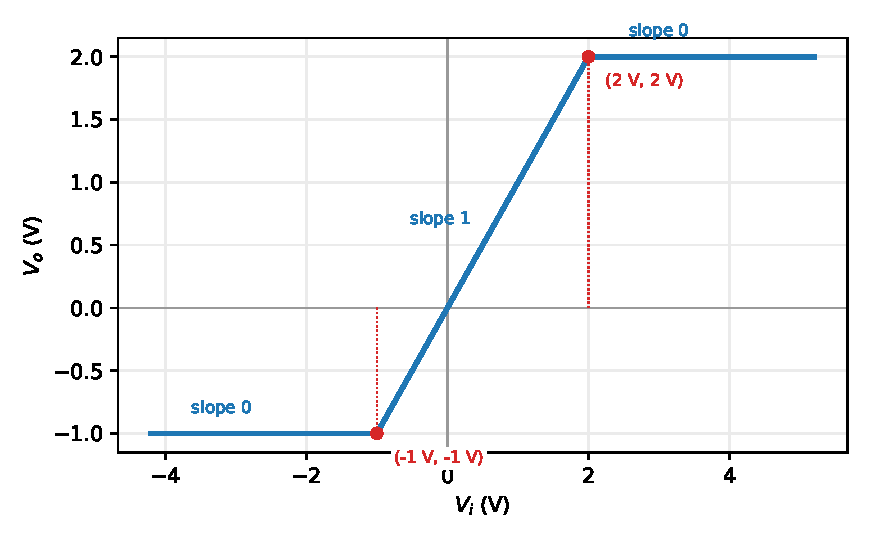
\includegraphics[width=0.62\linewidth,height=6cm,keepaspectratio]{p11_transfer}\end{center}
For $V_i(t) = 4\sin(2\pi\cdot 500\,t)$ simply pass every instant of $V_i(t)$ through the characteristic above (each piece is a straight line, so each part of the sinusoid is scaled and shifted):\begin{center}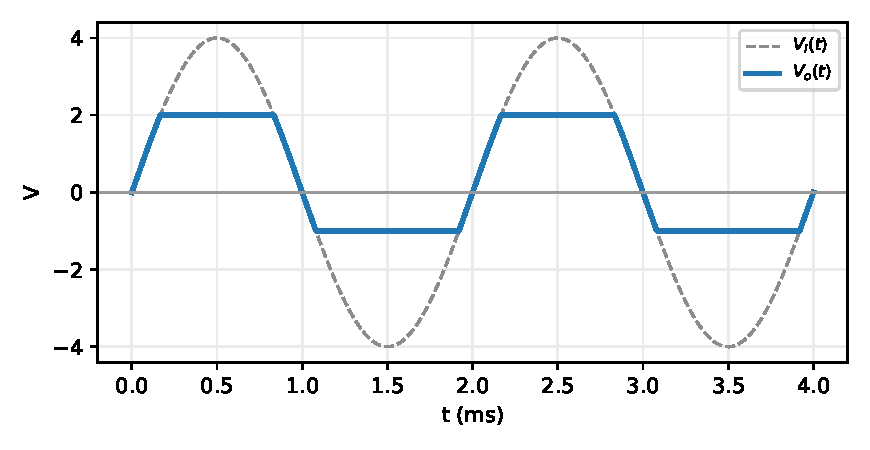
\includegraphics[width=0.62\linewidth,height=5cm,keepaspectratio]{p11_time}\end{center}

\begin{ansbox}
$V_o = \begin{cases} -1 & V_i < -1 \\ V_i & -1 < V_i < 2 \\ 2 & V_i > 2 \end{cases}$
\end{ansbox}

\newpage
\subsection*{Solution 3A.12 \hfill Medium}
\begin{center}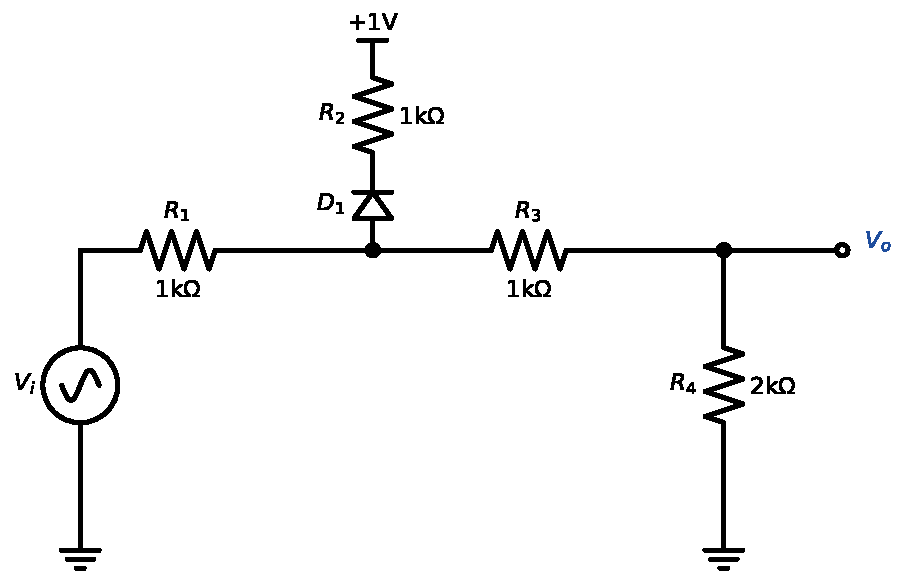
\includegraphics[width=0.9\linewidth,height=5cm,keepaspectratio]{p12_circuit}\end{center}
\solstep{1}{Model and method}Use the constant-voltage-drop model (tool T1): an OFF diode is an open circuit and needs $V_D<0.7$\,V; an ON diode is a $0.7$\,V source and needs $I_D>0$. With 1 diode there are $2$ ON/OFF combinations. For each one the circuit is linear: solve it with $V_i$ kept as a symbol, then check its assumptions --- each check is a condition on $V_i$ (tool T2). Node names used below: $V_{1}$ = node joining $D_{1}, R_{1}, R_{3}$; $V_{a}$ = node joining $D_{1}, R_{2}$.
\solstep{2}{Assume $D_{1}$ OFF}Replace $D_{1}$ OFF: an open circuit.

Equations (KCL at every node that is not an op-amp output, plus the diode voltages):\begin{align*}
&\text{KCL at }V_{1}: && \frac{V_{1} - V_i}{R_{1}} + \frac{V_{1} - V_{o}}{R_{3}} = 0 \\
&\text{KCL at }V_{a}: && \frac{V_{a} - 1}{R_{2}} = 0 \\
&\text{KCL at }V_{o}: && \frac{V_{o} - V_{1}}{R_{3}} + \frac{V_{o}}{R_{4}} = 0
\end{align*}


Solving these linear equations (substitute one into the other, as in Lecture 2) gives, with $V_i$ kept as a symbol:\begin{align*}
V_{o} &= 0.5V_i \\
V_{D_{1}} = V_{1} - V_{a} &= 0.75V_i - 1
\end{align*}


Check the assumptions: $V_{D_{1}} < 0.7$ $\Rightarrow$ $V_i < 2.267$\,V. So this state holds for $\boxed{V_i < 2.267}$, where $V_o = 0.5V_i$.
\solstep{3}{Assume $D_{1}$ ON}Replace $D_{1}$ ON: a $0.7$\,V source ($V_{1} - V_{a} = 0.7$) carrying an unknown current $I_{D_{1}}$ from anode to cathode.

Equations (KCL at every node that is not an op-amp output, plus the diode voltages):\begin{align*}
&\text{KCL at }V_{1}: && \frac{V_{1} - V_i}{R_{1}} + \frac{V_{1} - V_{o}}{R_{3}} + I_{D_{1}} = 0 \\
&\text{KCL at }V_{a}: && \frac{V_{a} - 1}{R_{2}} - I_{D_{1}} = 0 \\
&\text{KCL at }V_{o}: && \frac{V_{o} - V_{1}}{R_{3}} + \frac{V_{o}}{R_{4}} = 0 \\
&\text{D1 ON}: && V_{1} - V_{a} = 0.7
\end{align*}


Solving these linear equations (substitute one into the other, as in Lecture 2) gives, with $V_i$ kept as a symbol:\begin{align*}
V_{o} &= 0.2857V_i + 0.4857 \\
I_{D_{1}} &= 0.4286V_i - 0.9714\ \mathrm{mA}
\end{align*}


Check the assumptions: $I_{D_{1}} > 0$ $\Rightarrow$ $V_i > 2.267$\,V. So this state holds for $\boxed{V_i > 2.267}$, where $V_o = 0.2857V_i + 0.4857$.
\solstep{4}{Assemble and sketch}Put the valid states together:\[
V_o = \begin{cases} 0.5V_i & V_i < 2.267 \\ 0.2857V_i + 0.4857 & V_i > 2.267 \end{cases}
\]
Check: the pieces must meet at each breakpoint --- at $V_i=2.267$\,V both pieces give $V_o=1.133$\,V. \checkmark\begin{center}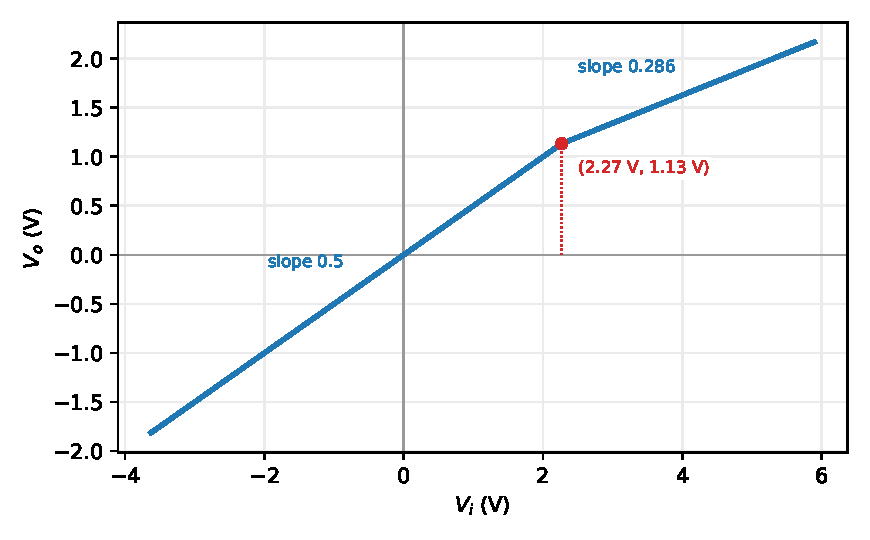
\includegraphics[width=0.62\linewidth,height=6cm,keepaspectratio]{p12_transfer}\end{center}

\begin{ansbox}
$V_o = \begin{cases} 0.5V_i & V_i < 2.267 \\ 0.2857V_i + 0.4857 & V_i > 2.267 \end{cases}$
\end{ansbox}

\newpage
\subsection*{Solution 3A.13 \hfill Hard}
\begin{center}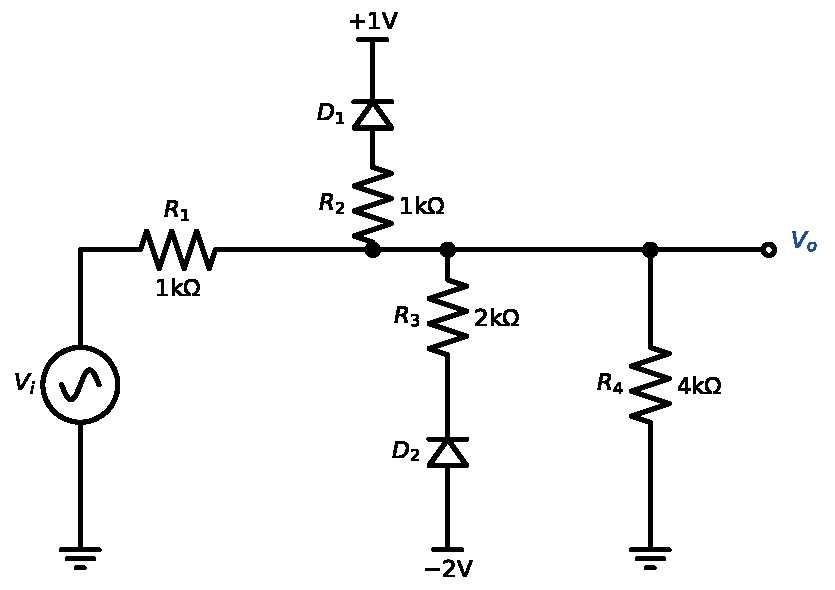
\includegraphics[width=0.9\linewidth,height=5cm,keepaspectratio]{p13_circuit}\end{center}
\solstep{1}{Model and method}Use the constant-voltage-drop model (tool T1): an OFF diode is an open circuit and needs $V_D<0.7$\,V; an ON diode is a $0.7$\,V source and needs $I_D>0$. With 2 diodes there are $4$ ON/OFF combinations. For each one the circuit is linear: solve it with $V_i$ kept as a symbol, then check its assumptions --- each check is a condition on $V_i$ (tool T2). Node names used below: $V_{a}$ = node joining $D_{1}, R_{2}$; $V_{b}$ = node joining $D_{2}, R_{3}$.
\solstep{2}{Assume $D_{1}$ OFF, $D_{2}$ ON}Replace $D_{1}$ OFF: an open circuit; $D_{2}$ ON: a $0.7$\,V source ($-2 - V_{b} = 0.7$) carrying an unknown current $I_{D_{2}}$ from anode to cathode.

Equations (KCL at every node that is not an op-amp output, plus the diode voltages):\begin{align*}
&\text{KCL at }V_{a}: && \frac{V_{a} - V_{o}}{R_{2}} = 0 \\
&\text{KCL at }V_{b}: && \frac{V_{b} - V_{o}}{R_{3}} - I_{D_{2}} = 0 \\
&\text{KCL at }V_{o}: && \frac{V_{o} - V_i}{R_{1}} + \frac{V_{o} - V_{a}}{R_{2}} + \frac{V_{o} - V_{b}}{R_{3}} + \frac{V_{o}}{R_{4}} = 0 \\
&\text{D2 ON}: && -2 - V_{b} = 0.7
\end{align*}


Solving these linear equations (substitute one into the other, as in Lecture 2) gives, with $V_i$ kept as a symbol:\begin{align*}
V_{o} &= 0.5714V_i - 0.7714 \\
V_{D_{1}} = V_{a} - 1 &= 0.5714V_i - 1.771 \\
I_{D_{2}} &= -0.2857V_i - 0.9643\ \mathrm{mA}
\end{align*}


Check the assumptions: $V_{D_{1}} < 0.7$ $\Rightarrow$ $V_i < 4.325$\,V; $I_{D_{2}} > 0$ $\Rightarrow$ $V_i < -3.375$\,V. So this state holds for $\boxed{V_i < -3.375}$, where $V_o = 0.5714V_i - 0.7714$.
\solstep{3}{Assume $D_{1}$ OFF, $D_{2}$ OFF}Replace $D_{1}$ OFF: an open circuit; $D_{2}$ OFF: an open circuit.

Equations (KCL at every node that is not an op-amp output, plus the diode voltages):\begin{align*}
&\text{KCL at }V_{a}: && \frac{V_{a} - V_{o}}{R_{2}} = 0 \\
&\text{KCL at }V_{b}: && \frac{V_{b} - V_{o}}{R_{3}} = 0 \\
&\text{KCL at }V_{o}: && \frac{V_{o} - V_i}{R_{1}} + \frac{V_{o} - V_{a}}{R_{2}} + \frac{V_{o} - V_{b}}{R_{3}} + \frac{V_{o}}{R_{4}} = 0
\end{align*}


Solving these linear equations (substitute one into the other, as in Lecture 2) gives, with $V_i$ kept as a symbol:\begin{align*}
V_{o} &= 0.8V_i \\
V_{D_{1}} = V_{a} - 1 &= 0.8V_i - 1 \\
V_{D_{2}} = -2 - V_{b} &= -0.8V_i - 2
\end{align*}


Check the assumptions: $V_{D_{1}} < 0.7$ $\Rightarrow$ $V_i < 2.125$\,V; $V_{D_{2}} < 0.7$ $\Rightarrow$ $V_i > -3.375$\,V. So this state holds for $\boxed{-3.375 < V_i < 2.125}$, where $V_o = 0.8V_i$.
\solstep{4}{Assume $D_{1}$ ON, $D_{2}$ OFF}Replace $D_{1}$ ON: a $0.7$\,V source ($V_{a} - 1 = 0.7$) carrying an unknown current $I_{D_{1}}$ from anode to cathode; $D_{2}$ OFF: an open circuit.

Equations (KCL at every node that is not an op-amp output, plus the diode voltages):\begin{align*}
&\text{KCL at }V_{a}: && \frac{V_{a} - V_{o}}{R_{2}} + I_{D_{1}} = 0 \\
&\text{KCL at }V_{b}: && \frac{V_{b} - V_{o}}{R_{3}} = 0 \\
&\text{KCL at }V_{o}: && \frac{V_{o} - V_i}{R_{1}} + \frac{V_{o} - V_{a}}{R_{2}} + \frac{V_{o} - V_{b}}{R_{3}} + \frac{V_{o}}{R_{4}} = 0 \\
&\text{D1 ON}: && V_{a} - 1 = 0.7
\end{align*}


Solving these linear equations (substitute one into the other, as in Lecture 2) gives, with $V_i$ kept as a symbol:\begin{align*}
V_{o} &= 0.4444V_i + 0.7556 \\
I_{D_{1}} &= 0.4444V_i - 0.9444\ \mathrm{mA} \\
V_{D_{2}} = -2 - V_{b} &= -0.4444V_i - 2.756
\end{align*}


Check the assumptions: $I_{D_{1}} > 0$ $\Rightarrow$ $V_i > 2.125$\,V; $V_{D_{2}} < 0.7$ $\Rightarrow$ $V_i > -7.775$\,V. So this state holds for $\boxed{V_i > 2.125}$, where $V_o = 0.4444V_i + 0.7556$.
\solstep{5}{The other combinations}\begin{itemize}[leftmargin=*,itemsep=2pt]
\item $D_{1}$ ON, $D_{2}$ ON: $I_{D_{1}}>0$ needs $V_i > 4.325$; $I_{D_{2}}>0$ needs $V_i < -7.775$ --- these cannot all hold, so this state never occurs.
\end{itemize}

\solstep{6}{Assemble and sketch}Put the valid states together:\[
V_o = \begin{cases} 0.5714V_i - 0.7714 & V_i < -3.375 \\ 0.8V_i & -3.375 < V_i < 2.125 \\ 0.4444V_i + 0.7556 & V_i > 2.125 \end{cases}
\]
Check: the pieces must meet at each breakpoint --- at $V_i=-3.375$\,V both pieces give $V_o=-2.7$\,V; at $V_i=2.125$\,V both pieces give $V_o=1.7$\,V. \checkmark\begin{center}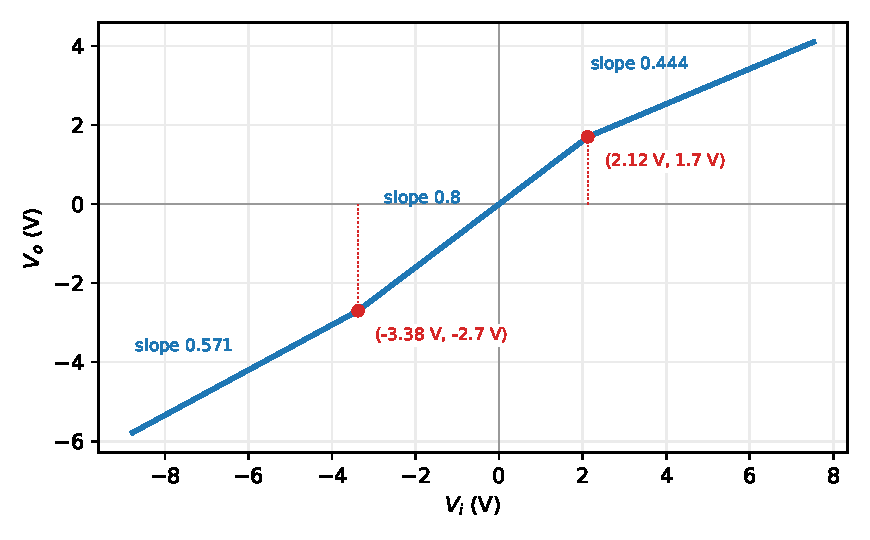
\includegraphics[width=0.62\linewidth,height=6cm,keepaspectratio]{p13_transfer}\end{center}
For $V_i(t) = 6\sin(2\pi\cdot 1000\,t)$ simply pass every instant of $V_i(t)$ through the characteristic above (each piece is a straight line, so each part of the sinusoid is scaled and shifted):\begin{center}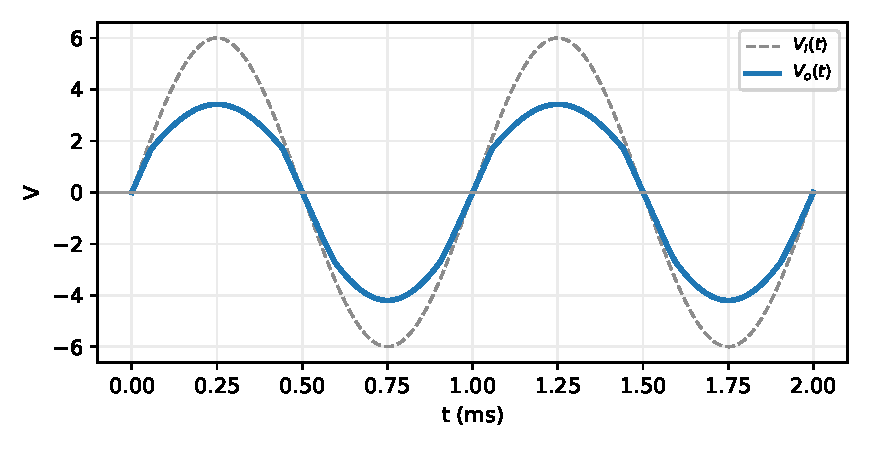
\includegraphics[width=0.62\linewidth,height=5cm,keepaspectratio]{p13_time}\end{center}

\begin{ansbox}
$V_o = \begin{cases} 0.5714V_i - 0.7714 & V_i < -3.375 \\ 0.8V_i & -3.375 < V_i < 2.125 \\ 0.4444V_i + 0.7556 & V_i > 2.125 \end{cases}$
\end{ansbox}

\newpage
\subsection*{Solution 3A.14 \hfill Hard}
\begin{center}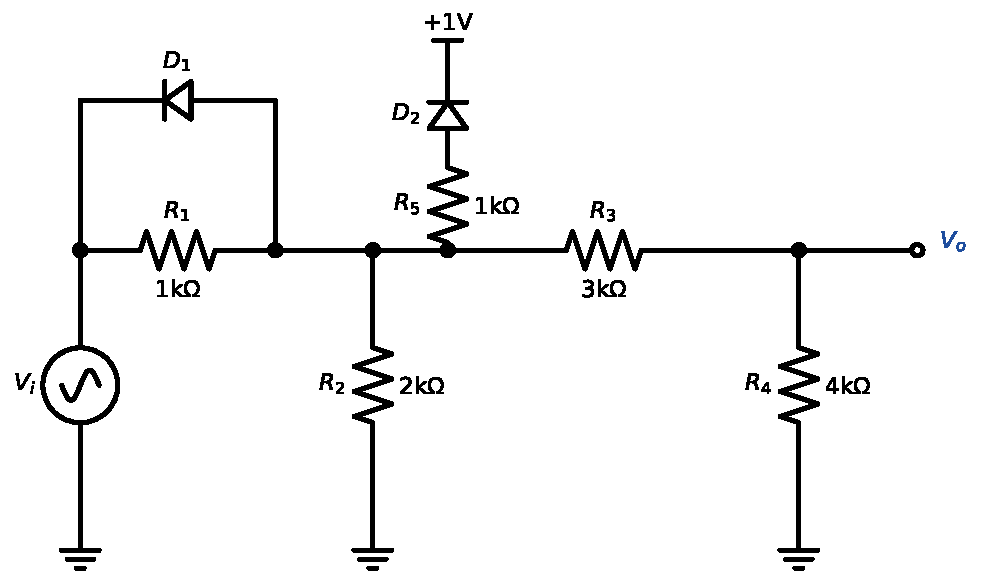
\includegraphics[width=0.9\linewidth,height=5cm,keepaspectratio]{p14_circuit}\end{center}
\solstep{1}{Model and method}Use the constant-voltage-drop model (tool T1): an OFF diode is an open circuit and needs $V_D<0.7$\,V; an ON diode is a $0.7$\,V source and needs $I_D>0$. With 2 diodes there are $4$ ON/OFF combinations. For each one the circuit is linear: solve it with $V_i$ kept as a symbol, then check its assumptions --- each check is a condition on $V_i$ (tool T2). Node names used below: $V_{1}$ = node joining $D_{1}, R_{1}, R_{2}, R_{3}, R_{5}$; $V_{a}$ = node joining $D_{2}, R_{5}$.
\solstep{2}{Assume $D_{1}$ ON, $D_{2}$ OFF}Replace $D_{1}$ ON: a $0.7$\,V source ($V_{1} - V_i = 0.7$) carrying an unknown current $I_{D_{1}}$ from anode to cathode; $D_{2}$ OFF: an open circuit.

Equations (KCL at every node that is not an op-amp output, plus the diode voltages):\begin{align*}
&\text{KCL at }V_{1}: && \frac{V_{1} - V_i}{R_{1}} + \frac{V_{1}}{R_{2}} + \frac{V_{1} - V_{a}}{R_{5}} + \frac{V_{1} - V_{o}}{R_{3}} + I_{D_{1}} = 0 \\
&\text{KCL at }V_{a}: && \frac{V_{a} - V_{1}}{R_{5}} = 0 \\
&\text{KCL at }V_{o}: && \frac{V_{o} - V_{1}}{R_{3}} + \frac{V_{o}}{R_{4}} = 0 \\
&\text{D1 ON}: && V_{1} - V_i = 0.7
\end{align*}


Solving these linear equations (substitute one into the other, as in Lecture 2) gives, with $V_i$ kept as a symbol:\begin{align*}
V_{o} &= 0.5714V_i + 0.4 \\
I_{D_{1}} &= -0.6429V_i - 1.15\ \mathrm{mA} \\
V_{D_{2}} = V_{a} - 1 &= V_i - 0.3
\end{align*}


Check the assumptions: $I_{D_{1}} > 0$ $\Rightarrow$ $V_i < -1.789$\,V; $V_{D_{2}} < 0.7$ $\Rightarrow$ $V_i < 1$\,V. So this state holds for $\boxed{V_i < -1.789}$, where $V_o = 0.5714V_i + 0.4$.
\solstep{3}{Assume $D_{1}$ OFF, $D_{2}$ OFF}Replace $D_{1}$ OFF: an open circuit; $D_{2}$ OFF: an open circuit.

Equations (KCL at every node that is not an op-amp output, plus the diode voltages):\begin{align*}
&\text{KCL at }V_{1}: && \frac{V_{1} - V_i}{R_{1}} + \frac{V_{1}}{R_{2}} + \frac{V_{1} - V_{a}}{R_{5}} + \frac{V_{1} - V_{o}}{R_{3}} = 0 \\
&\text{KCL at }V_{a}: && \frac{V_{a} - V_{1}}{R_{5}} = 0 \\
&\text{KCL at }V_{o}: && \frac{V_{o} - V_{1}}{R_{3}} + \frac{V_{o}}{R_{4}} = 0
\end{align*}


Solving these linear equations (substitute one into the other, as in Lecture 2) gives, with $V_i$ kept as a symbol:\begin{align*}
V_{o} &= 0.3478V_i \\
V_{D_{1}} = V_{1} - V_i &= -0.3913V_i \\
V_{D_{2}} = V_{a} - 1 &= 0.6087V_i - 1
\end{align*}


Check the assumptions: $V_{D_{1}} < 0.7$ $\Rightarrow$ $V_i > -1.789$\,V; $V_{D_{2}} < 0.7$ $\Rightarrow$ $V_i < 2.793$\,V. So this state holds for $\boxed{-1.789 < V_i < 2.793}$, where $V_o = 0.3478V_i$.
\solstep{4}{Assume $D_{1}$ OFF, $D_{2}$ ON}Replace $D_{1}$ OFF: an open circuit; $D_{2}$ ON: a $0.7$\,V source ($V_{a} - 1 = 0.7$) carrying an unknown current $I_{D_{2}}$ from anode to cathode.

Equations (KCL at every node that is not an op-amp output, plus the diode voltages):\begin{align*}
&\text{KCL at }V_{1}: && \frac{V_{1} - V_i}{R_{1}} + \frac{V_{1}}{R_{2}} + \frac{V_{1} - V_{a}}{R_{5}} + \frac{V_{1} - V_{o}}{R_{3}} = 0 \\
&\text{KCL at }V_{a}: && \frac{V_{a} - V_{1}}{R_{5}} + I_{D_{2}} = 0 \\
&\text{KCL at }V_{o}: && \frac{V_{o} - V_{1}}{R_{3}} + \frac{V_{o}}{R_{4}} = 0 \\
&\text{D2 ON}: && V_{a} - 1 = 0.7
\end{align*}


Solving these linear equations (substitute one into the other, as in Lecture 2) gives, with $V_i$ kept as a symbol:\begin{align*}
V_{o} &= 0.2162V_i + 0.3676 \\
V_{D_{1}} = V_{1} - V_i &= -0.6216V_i + 0.6432 \\
I_{D_{2}} &= 0.3784V_i - 1.057\ \mathrm{mA}
\end{align*}


Check the assumptions: $V_{D_{1}} < 0.7$ $\Rightarrow$ $V_i > -0.0913$\,V; $I_{D_{2}} > 0$ $\Rightarrow$ $V_i > 2.793$\,V. So this state holds for $\boxed{V_i > 2.793}$, where $V_o = 0.2162V_i + 0.3676$.
\solstep{5}{The other combinations}\begin{itemize}[leftmargin=*,itemsep=2pt]
\item $D_{1}$ ON, $D_{2}$ ON: $I_{D_{1}}>0$ needs $V_i < -0.0913$; $I_{D_{2}}>0$ needs $V_i > 1$ --- these cannot all hold, so this state never occurs.
\end{itemize}

\solstep{6}{Assemble and sketch}Put the valid states together:\[
V_o = \begin{cases} 0.5714V_i + 0.4 & V_i < -1.789 \\ 0.3478V_i & -1.789 < V_i < 2.793 \\ 0.2162V_i + 0.3676 & V_i > 2.793 \end{cases}
\]
Check: the pieces must meet at each breakpoint --- at $V_i=-1.789$\,V both pieces give $V_o=-0.6222$\,V; at $V_i=2.793$\,V both pieces give $V_o=0.9714$\,V. \checkmark\begin{center}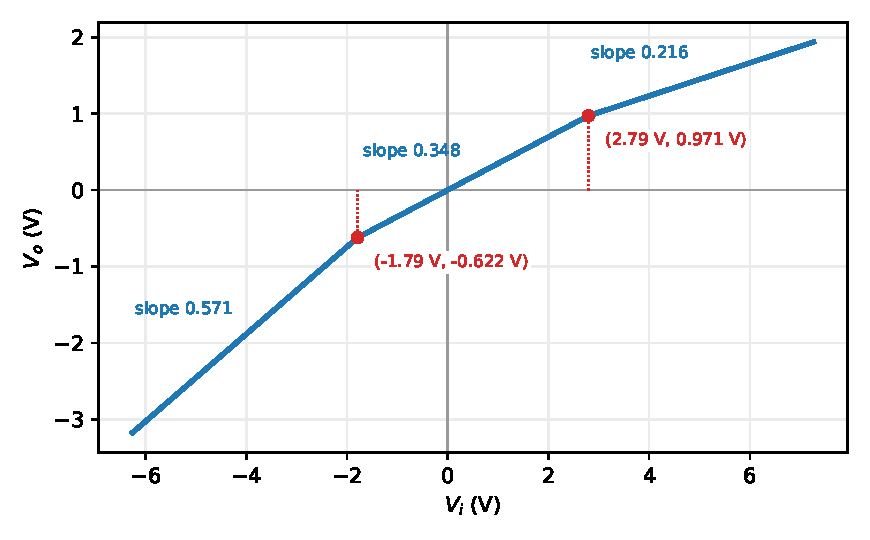
\includegraphics[width=0.62\linewidth,height=6cm,keepaspectratio]{p14_transfer}\end{center}

\begin{ansbox}
$V_o = \begin{cases} 0.5714V_i + 0.4 & V_i < -1.789 \\ 0.3478V_i & -1.789 < V_i < 2.793 \\ 0.2162V_i + 0.3676 & V_i > 2.793 \end{cases}$
\end{ansbox}

\newpage
\subsection*{Solution 3A.15 \hfill Hard}
\begin{center}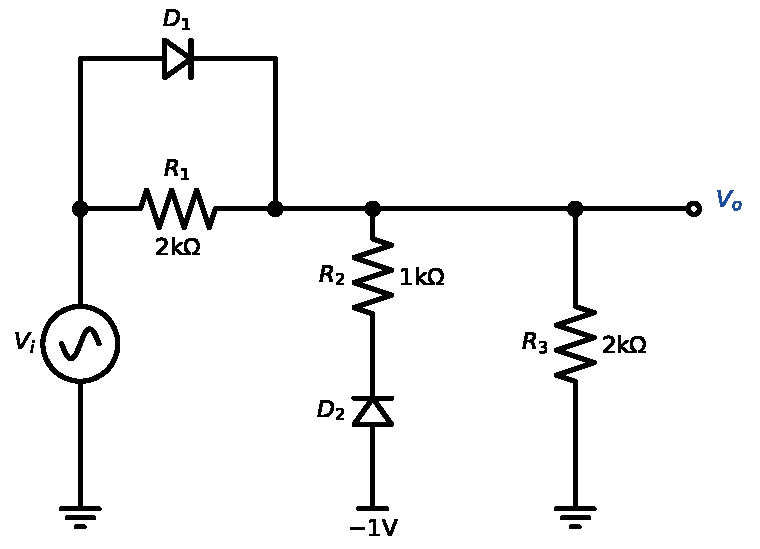
\includegraphics[width=0.9\linewidth,height=5cm,keepaspectratio]{p15_circuit}\end{center}
\solstep{1}{Model and method}Use the constant-voltage-drop model (tool T1): an OFF diode is an open circuit and needs $V_D<0.7$\,V; an ON diode is a $0.7$\,V source and needs $I_D>0$. With 2 diodes there are $4$ ON/OFF combinations. For each one the circuit is linear: solve it with $V_i$ kept as a symbol, then check its assumptions --- each check is a condition on $V_i$ (tool T2). Node names used below: $V_{a}$ = node joining $D_{2}, R_{2}$.
\solstep{2}{Assume $D_{1}$ OFF, $D_{2}$ ON}Replace $D_{1}$ OFF: an open circuit; $D_{2}$ ON: a $0.7$\,V source ($-1 - V_{a} = 0.7$) carrying an unknown current $I_{D_{2}}$ from anode to cathode.

Equations (KCL at every node that is not an op-amp output, plus the diode voltages):\begin{align*}
&\text{KCL at }V_{a}: && \frac{V_{a} - V_{o}}{R_{2}} - I_{D_{2}} = 0 \\
&\text{KCL at }V_{o}: && \frac{V_{o} - V_i}{R_{1}} + \frac{V_{o} - V_{a}}{R_{2}} + \frac{V_{o}}{R_{3}} = 0 \\
&\text{D2 ON}: && -1 - V_{a} = 0.7
\end{align*}


Solving these linear equations (substitute one into the other, as in Lecture 2) gives, with $V_i$ kept as a symbol:\begin{align*}
V_{o} &= 0.25V_i - 0.85 \\
V_{D_{1}} = V_i - V_{o} &= 0.75V_i + 0.85 \\
I_{D_{2}} &= -0.25V_i - 0.85\ \mathrm{mA}
\end{align*}


Check the assumptions: $V_{D_{1}} < 0.7$ $\Rightarrow$ $V_i < -0.2$\,V; $I_{D_{2}} > 0$ $\Rightarrow$ $V_i < -3.4$\,V. So this state holds for $\boxed{V_i < -3.4}$, where $V_o = 0.25V_i - 0.85$.
\solstep{3}{Assume $D_{1}$ OFF, $D_{2}$ OFF}Replace $D_{1}$ OFF: an open circuit; $D_{2}$ OFF: an open circuit.

Equations (KCL at every node that is not an op-amp output, plus the diode voltages):\begin{align*}
&\text{KCL at }V_{a}: && \frac{V_{a} - V_{o}}{R_{2}} = 0 \\
&\text{KCL at }V_{o}: && \frac{V_{o} - V_i}{R_{1}} + \frac{V_{o} - V_{a}}{R_{2}} + \frac{V_{o}}{R_{3}} = 0
\end{align*}


Solving these linear equations (substitute one into the other, as in Lecture 2) gives, with $V_i$ kept as a symbol:\begin{align*}
V_{o} &= 0.5V_i \\
V_{D_{1}} = V_i - V_{o} &= 0.5V_i \\
V_{D_{2}} = -1 - V_{a} &= -0.5V_i - 1
\end{align*}


Check the assumptions: $V_{D_{1}} < 0.7$ $\Rightarrow$ $V_i < 1.4$\,V; $V_{D_{2}} < 0.7$ $\Rightarrow$ $V_i > -3.4$\,V. So this state holds for $\boxed{-3.4 < V_i < 1.4}$, where $V_o = 0.5V_i$.
\solstep{4}{Assume $D_{1}$ ON, $D_{2}$ OFF}Replace $D_{1}$ ON: a $0.7$\,V source ($V_i - V_{o} = 0.7$) carrying an unknown current $I_{D_{1}}$ from anode to cathode; $D_{2}$ OFF: an open circuit.

Equations (KCL at every node that is not an op-amp output, plus the diode voltages):\begin{align*}
&\text{KCL at }V_{a}: && \frac{V_{a} - V_{o}}{R_{2}} = 0 \\
&\text{KCL at }V_{o}: && \frac{V_{o} - V_i}{R_{1}} + \frac{V_{o} - V_{a}}{R_{2}} + \frac{V_{o}}{R_{3}} - I_{D_{1}} = 0 \\
&\text{D1 ON}: && V_i - V_{o} = 0.7
\end{align*}


Solving these linear equations (substitute one into the other, as in Lecture 2) gives, with $V_i$ kept as a symbol:\begin{align*}
V_{o} &= V_i - 0.7 \\
I_{D_{1}} &= 0.5V_i - 0.7\ \mathrm{mA} \\
V_{D_{2}} = -1 - V_{a} &= -V_i - 0.3
\end{align*}


Check the assumptions: $I_{D_{1}} > 0$ $\Rightarrow$ $V_i > 1.4$\,V; $V_{D_{2}} < 0.7$ $\Rightarrow$ $V_i > -1$\,V. So this state holds for $\boxed{V_i > 1.4}$, where $V_o = V_i - 0.7$.
\solstep{5}{The other combinations}\begin{itemize}[leftmargin=*,itemsep=2pt]
\item $D_{1}$ ON, $D_{2}$ ON: $I_{D_{1}}>0$ needs $V_i > -0.2$; $I_{D_{2}}>0$ needs $V_i < -1$ --- these cannot all hold, so this state never occurs.
\end{itemize}

\solstep{6}{Assemble and sketch}Put the valid states together:\[
V_o = \begin{cases} 0.25V_i - 0.85 & V_i < -3.4 \\ 0.5V_i & -3.4 < V_i < 1.4 \\ V_i - 0.7 & V_i > 1.4 \end{cases}
\]
Check: the pieces must meet at each breakpoint --- at $V_i=-3.4$\,V both pieces give $V_o=-1.7$\,V; at $V_i=1.4$\,V both pieces give $V_o=0.7$\,V. \checkmark\begin{center}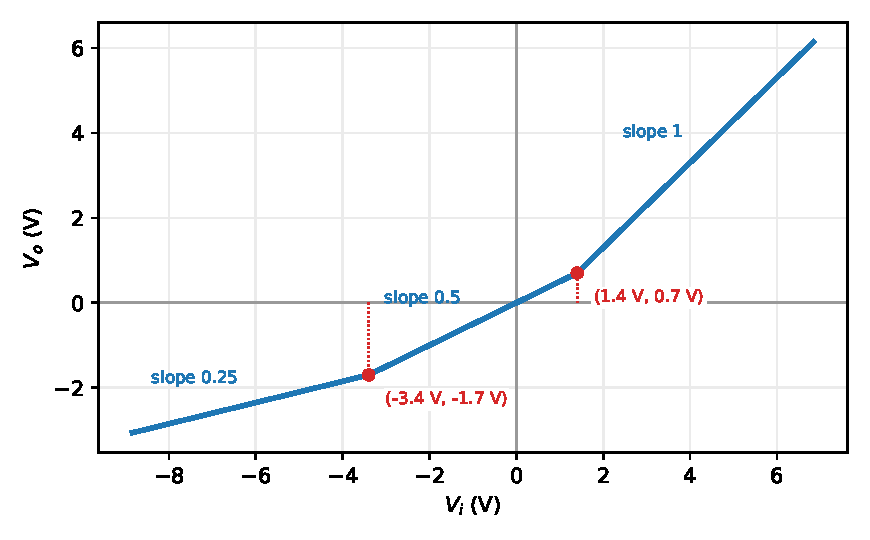
\includegraphics[width=0.62\linewidth,height=6cm,keepaspectratio]{p15_transfer}\end{center}

\begin{ansbox}
$V_o = \begin{cases} 0.25V_i - 0.85 & V_i < -3.4 \\ 0.5V_i & -3.4 < V_i < 1.4 \\ V_i - 0.7 & V_i > 1.4 \end{cases}$
\end{ansbox}

\newpage
\subsection*{Solution 3A.16 \hfill Hard}
\begin{center}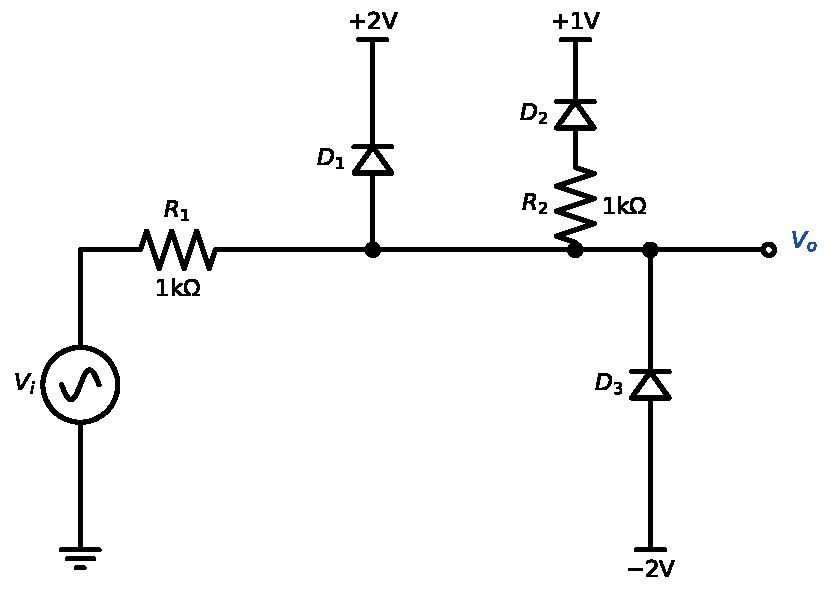
\includegraphics[width=0.9\linewidth,height=5cm,keepaspectratio]{p16_circuit}\end{center}
\solstep{1}{Model and method}Use the constant-voltage-drop model (tool T1): an OFF diode is an open circuit and needs $V_D<0.7$\,V; an ON diode is a $0.7$\,V source and needs $I_D>0$. With 3 diodes there are $8$ ON/OFF combinations. For each one the circuit is linear: solve it with $V_i$ kept as a symbol, then check its assumptions --- each check is a condition on $V_i$ (tool T2). Node names used below: $V_{a}$ = node joining $D_{2}, R_{2}$.
\solstep{2}{Assume $D_{1}$ OFF, $D_{2}$ OFF, $D_{3}$ ON}Replace $D_{1}$ OFF: an open circuit; $D_{2}$ OFF: an open circuit; $D_{3}$ ON: a $0.7$\,V source ($-2 - V_{o} = 0.7$) carrying an unknown current $I_{D_{3}}$ from anode to cathode.

Equations (KCL at every node that is not an op-amp output, plus the diode voltages):\begin{align*}
&\text{KCL at }V_{a}: && \frac{V_{a} - V_{o}}{R_{2}} = 0 \\
&\text{KCL at }V_{o}: && \frac{V_{o} - V_i}{R_{1}} + \frac{V_{o} - V_{a}}{R_{2}} - I_{D_{3}} = 0 \\
&\text{D3 ON}: && -2 - V_{o} = 0.7
\end{align*}


Solving these linear equations (substitute one into the other, as in Lecture 2) gives, with $V_i$ kept as a symbol:\begin{align*}
V_{o} &= -2.7 \\
V_{D_{1}} = V_{o} - 2 &= -4.7 \\
V_{D_{2}} = V_{a} - 1 &= -3.7 \\
I_{D_{3}} &= -V_i - 2.7\ \mathrm{mA}
\end{align*}


Check the assumptions: $V_{D_{1}} < 0.7$ $\Rightarrow$ true for every $V_i$; $V_{D_{2}} < 0.7$ $\Rightarrow$ true for every $V_i$; $I_{D_{3}} > 0$ $\Rightarrow$ $V_i < -2.7$\,V. So this state holds for $\boxed{V_i < -2.7}$, where $V_o = -2.7$.
\solstep{3}{Assume $D_{1}$ OFF, $D_{2}$ OFF, $D_{3}$ OFF}Replace $D_{1}$ OFF: an open circuit; $D_{2}$ OFF: an open circuit; $D_{3}$ OFF: an open circuit.

Equations (KCL at every node that is not an op-amp output, plus the diode voltages):\begin{align*}
&\text{KCL at }V_{a}: && \frac{V_{a} - V_{o}}{R_{2}} = 0 \\
&\text{KCL at }V_{o}: && \frac{V_{o} - V_i}{R_{1}} + \frac{V_{o} - V_{a}}{R_{2}} = 0
\end{align*}


Solving these linear equations (substitute one into the other, as in Lecture 2) gives, with $V_i$ kept as a symbol:\begin{align*}
V_{o} &= V_i \\
V_{D_{1}} = V_{o} - 2 &= V_i - 2 \\
V_{D_{2}} = V_{a} - 1 &= V_i - 1 \\
V_{D_{3}} = -2 - V_{o} &= -V_i - 2
\end{align*}


Check the assumptions: $V_{D_{1}} < 0.7$ $\Rightarrow$ $V_i < 2.7$\,V; $V_{D_{2}} < 0.7$ $\Rightarrow$ $V_i < 1.7$\,V; $V_{D_{3}} < 0.7$ $\Rightarrow$ $V_i > -2.7$\,V. So this state holds for $\boxed{-2.7 < V_i < 1.7}$, where $V_o = V_i$.
\solstep{4}{Assume $D_{1}$ OFF, $D_{2}$ ON, $D_{3}$ OFF}Replace $D_{1}$ OFF: an open circuit; $D_{2}$ ON: a $0.7$\,V source ($V_{a} - 1 = 0.7$) carrying an unknown current $I_{D_{2}}$ from anode to cathode; $D_{3}$ OFF: an open circuit.

Equations (KCL at every node that is not an op-amp output, plus the diode voltages):\begin{align*}
&\text{KCL at }V_{a}: && \frac{V_{a} - V_{o}}{R_{2}} + I_{D_{2}} = 0 \\
&\text{KCL at }V_{o}: && \frac{V_{o} - V_i}{R_{1}} + \frac{V_{o} - V_{a}}{R_{2}} = 0 \\
&\text{D2 ON}: && V_{a} - 1 = 0.7
\end{align*}


Solving these linear equations (substitute one into the other, as in Lecture 2) gives, with $V_i$ kept as a symbol:\begin{align*}
V_{o} &= 0.5V_i + 0.85 \\
V_{D_{1}} = V_{o} - 2 &= 0.5V_i - 1.15 \\
I_{D_{2}} &= 0.5V_i - 0.85\ \mathrm{mA} \\
V_{D_{3}} = -2 - V_{o} &= -0.5V_i - 2.85
\end{align*}


Check the assumptions: $V_{D_{1}} < 0.7$ $\Rightarrow$ $V_i < 3.7$\,V; $I_{D_{2}} > 0$ $\Rightarrow$ $V_i > 1.7$\,V; $V_{D_{3}} < 0.7$ $\Rightarrow$ $V_i > -7.1$\,V. So this state holds for $\boxed{1.7 < V_i < 3.7}$, where $V_o = 0.5V_i + 0.85$.
\solstep{5}{Assume $D_{1}$ ON, $D_{2}$ ON, $D_{3}$ OFF}Replace $D_{1}$ ON: a $0.7$\,V source ($V_{o} - 2 = 0.7$) carrying an unknown current $I_{D_{1}}$ from anode to cathode; $D_{2}$ ON: a $0.7$\,V source ($V_{a} - 1 = 0.7$) carrying an unknown current $I_{D_{2}}$ from anode to cathode; $D_{3}$ OFF: an open circuit.

Equations (KCL at every node that is not an op-amp output, plus the diode voltages):\begin{align*}
&\text{KCL at }V_{a}: && \frac{V_{a} - V_{o}}{R_{2}} + I_{D_{2}} = 0 \\
&\text{KCL at }V_{o}: && \frac{V_{o} - V_i}{R_{1}} + \frac{V_{o} - V_{a}}{R_{2}} + I_{D_{1}} = 0 \\
&\text{D1 ON}: && V_{o} - 2 = 0.7 \\
&\text{D2 ON}: && V_{a} - 1 = 0.7
\end{align*}


Solving these linear equations (substitute one into the other, as in Lecture 2) gives, with $V_i$ kept as a symbol:\begin{align*}
V_{o} &= 2.7 \\
I_{D_{1}} &= V_i - 3.7\ \mathrm{mA} \\
I_{D_{2}} &= 1\ \mathrm{mA} \\
V_{D_{3}} = -2 - V_{o} &= -4.7
\end{align*}


Check the assumptions: $I_{D_{1}} > 0$ $\Rightarrow$ $V_i > 3.7$\,V; $I_{D_{2}} > 0$ $\Rightarrow$ true for every $V_i$; $V_{D_{3}} < 0.7$ $\Rightarrow$ true for every $V_i$. So this state holds for $\boxed{V_i > 3.7}$, where $V_o = 2.7$.
\solstep{6}{The other combinations}\begin{itemize}[leftmargin=*,itemsep=2pt]
\item $D_{1}$ OFF, $D_{2}$ ON, $D_{3}$ ON: $V_{D_{1}}<0.7$ is always true; $I_{D_{2}}>0$ is never true; $I_{D_{3}}>0$ needs $V_i < -7.1$ --- these cannot all hold, so this state never occurs.
\item $D_{1}$ ON, $D_{2}$ OFF, $D_{3}$ OFF: $I_{D_{1}}>0$ needs $V_i > 2.7$; $V_{D_{2}}<0.7$ is never true; $V_{D_{3}}<0.7$ is always true --- these cannot all hold, so this state never occurs.
\item $D_{1}$ ON, $D_{2}$ OFF, $D_{3}$ ON: the ON diodes would have to hold the same node at two different voltages at once, which no circuit can do --- these cannot all hold, so this state never occurs.
\item $D_{1}$ ON, $D_{2}$ ON, $D_{3}$ ON: the ON diodes would have to hold the same node at two different voltages at once, which no circuit can do --- these cannot all hold, so this state never occurs.
\end{itemize}

\solstep{7}{Assemble and sketch}Put the valid states together:\[
V_o = \begin{cases} -2.7 & V_i < -2.7 \\ V_i & -2.7 < V_i < 1.7 \\ 0.5V_i + 0.85 & 1.7 < V_i < 3.7 \\ 2.7 & V_i > 3.7 \end{cases}
\]
Check: the pieces must meet at each breakpoint --- at $V_i=-2.7$\,V both pieces give $V_o=-2.7$\,V; at $V_i=1.7$\,V both pieces give $V_o=1.7$\,V; at $V_i=3.7$\,V both pieces give $V_o=2.7$\,V. \checkmark\begin{center}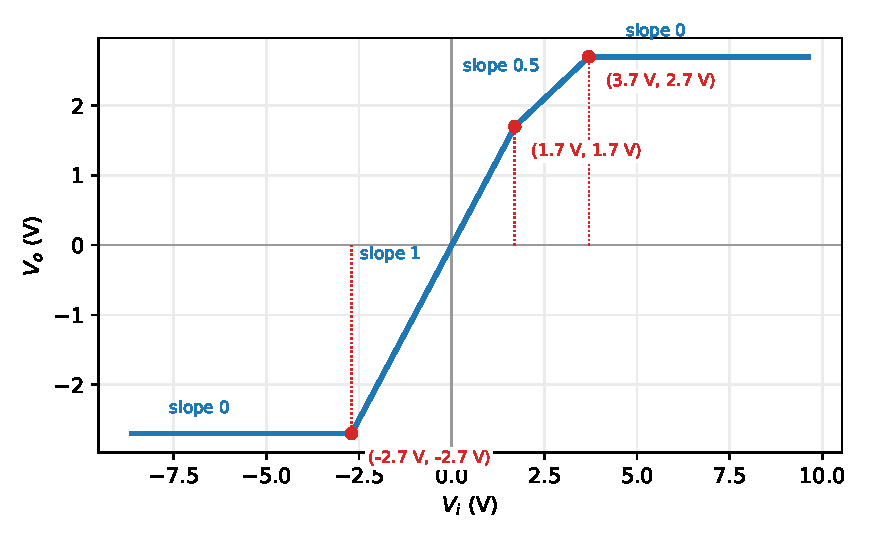
\includegraphics[width=0.62\linewidth,height=6cm,keepaspectratio]{p16_transfer}\end{center}
For $V_i(t) = 5\sin(2\pi\cdot 1000\,t)$ simply pass every instant of $V_i(t)$ through the characteristic above (each piece is a straight line, so each part of the sinusoid is scaled and shifted):\begin{center}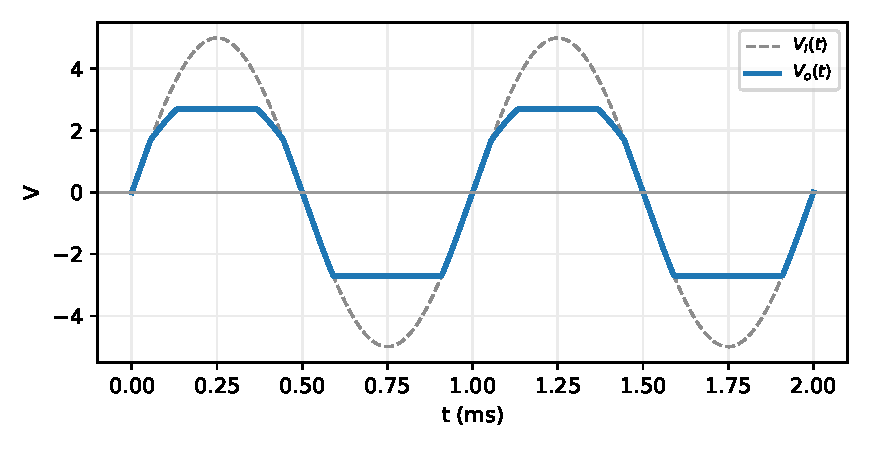
\includegraphics[width=0.62\linewidth,height=5cm,keepaspectratio]{p16_time}\end{center}

\begin{ansbox}
$V_o = \begin{cases} -2.7 & V_i < -2.7 \\ V_i & -2.7 < V_i < 1.7 \\ 0.5V_i + 0.85 & 1.7 < V_i < 3.7 \\ 2.7 & V_i > 3.7 \end{cases}$
\end{ansbox}

\newpage
\subsection*{Solution 3A.17 \hfill Hard}
\begin{center}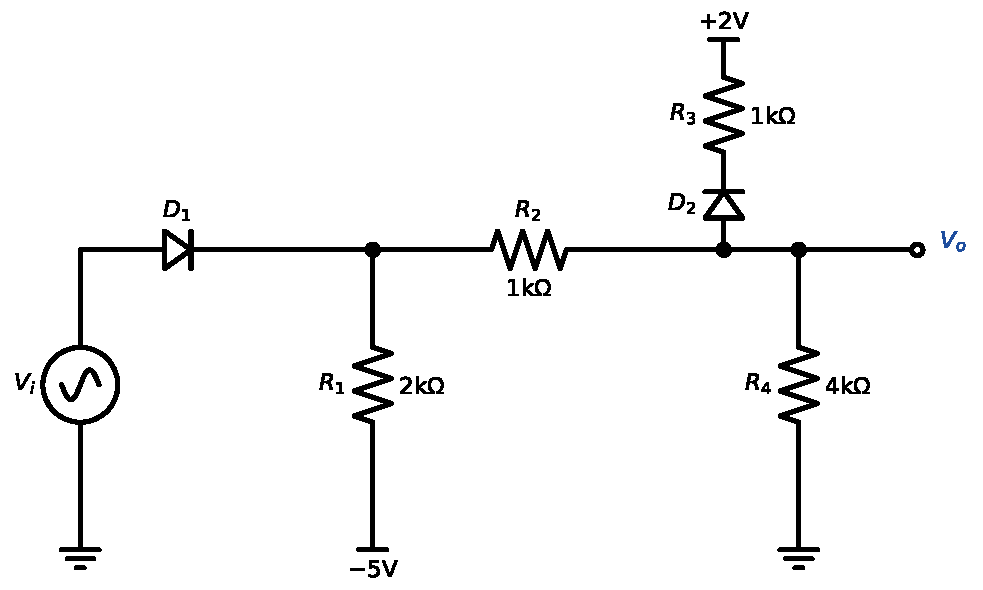
\includegraphics[width=0.9\linewidth,height=5cm,keepaspectratio]{p17_circuit}\end{center}
\solstep{1}{Model and method}Use the constant-voltage-drop model (tool T1): an OFF diode is an open circuit and needs $V_D<0.7$\,V; an ON diode is a $0.7$\,V source and needs $I_D>0$. With 2 diodes there are $4$ ON/OFF combinations. For each one the circuit is linear: solve it with $V_i$ kept as a symbol, then check its assumptions --- each check is a condition on $V_i$ (tool T2). Node names used below: $V_{1}$ = node joining $D_{1}, R_{1}, R_{2}$; $V_{a}$ = node joining $D_{2}, R_{3}$.
\solstep{2}{Assume $D_{1}$ OFF, $D_{2}$ OFF}Replace $D_{1}$ OFF: an open circuit; $D_{2}$ OFF: an open circuit.

Equations (KCL at every node that is not an op-amp output, plus the diode voltages):\begin{align*}
&\text{KCL at }V_{1}: && \frac{V_{1} - -5}{R_{1}} + \frac{V_{1} - V_{o}}{R_{2}} = 0 \\
&\text{KCL at }V_{a}: && \frac{V_{a} - 2}{R_{3}} = 0 \\
&\text{KCL at }V_{o}: && \frac{V_{o} - V_{1}}{R_{2}} + \frac{V_{o}}{R_{4}} = 0
\end{align*}


Solving these linear equations (substitute one into the other, as in Lecture 2) gives, with $V_i$ kept as a symbol:\begin{align*}
V_{o} &= -2.857 \\
V_{D_{1}} = V_i - V_{1} &= V_i + 3.571 \\
V_{D_{2}} = V_{o} - V_{a} &= -4.857
\end{align*}


Check the assumptions: $V_{D_{1}} < 0.7$ $\Rightarrow$ $V_i < -2.871$\,V; $V_{D_{2}} < 0.7$ $\Rightarrow$ true for every $V_i$. So this state holds for $\boxed{V_i < -2.871}$, where $V_o = -2.857$.
\solstep{3}{Assume $D_{1}$ ON, $D_{2}$ OFF}Replace $D_{1}$ ON: a $0.7$\,V source ($V_i - V_{1} = 0.7$) carrying an unknown current $I_{D_{1}}$ from anode to cathode; $D_{2}$ OFF: an open circuit.

Equations (KCL at every node that is not an op-amp output, plus the diode voltages):\begin{align*}
&\text{KCL at }V_{1}: && \frac{V_{1} - -5}{R_{1}} + \frac{V_{1} - V_{o}}{R_{2}} - I_{D_{1}} = 0 \\
&\text{KCL at }V_{a}: && \frac{V_{a} - 2}{R_{3}} = 0 \\
&\text{KCL at }V_{o}: && \frac{V_{o} - V_{1}}{R_{2}} + \frac{V_{o}}{R_{4}} = 0 \\
&\text{D1 ON}: && V_i - V_{1} = 0.7
\end{align*}


Solving these linear equations (substitute one into the other, as in Lecture 2) gives, with $V_i$ kept as a symbol:\begin{align*}
V_{o} &= 0.8V_i - 0.56 \\
I_{D_{1}} &= 0.7V_i + 2.01\ \mathrm{mA} \\
V_{D_{2}} = V_{o} - V_{a} &= 0.8V_i - 2.56
\end{align*}


Check the assumptions: $I_{D_{1}} > 0$ $\Rightarrow$ $V_i > -2.871$\,V; $V_{D_{2}} < 0.7$ $\Rightarrow$ $V_i < 4.075$\,V. So this state holds for $\boxed{-2.871 < V_i < 4.075}$, where $V_o = 0.8V_i - 0.56$.
\solstep{4}{Assume $D_{1}$ ON, $D_{2}$ ON}Replace $D_{1}$ ON: a $0.7$\,V source ($V_i - V_{1} = 0.7$) carrying an unknown current $I_{D_{1}}$ from anode to cathode; $D_{2}$ ON: a $0.7$\,V source ($V_{o} - V_{a} = 0.7$) carrying an unknown current $I_{D_{2}}$ from anode to cathode.

Equations (KCL at every node that is not an op-amp output, plus the diode voltages):\begin{align*}
&\text{KCL at }V_{1}: && \frac{V_{1} - -5}{R_{1}} + \frac{V_{1} - V_{o}}{R_{2}} - I_{D_{1}} = 0 \\
&\text{KCL at }V_{a}: && \frac{V_{a} - 2}{R_{3}} - I_{D_{2}} = 0 \\
&\text{KCL at }V_{o}: && \frac{V_{o} - V_{1}}{R_{2}} + \frac{V_{o}}{R_{4}} + I_{D_{2}} = 0 \\
&\text{D1 ON}: && V_i - V_{1} = 0.7 \\
&\text{D2 ON}: && V_{o} - V_{a} = 0.7
\end{align*}


Solving these linear equations (substitute one into the other, as in Lecture 2) gives, with $V_i$ kept as a symbol:\begin{align*}
V_{o} &= 0.4444V_i + 0.8889 \\
I_{D_{1}} &= 1.056V_i + 0.5611\ \mathrm{mA} \\
I_{D_{2}} &= 0.4444V_i - 1.811\ \mathrm{mA}
\end{align*}


Check the assumptions: $I_{D_{1}} > 0$ $\Rightarrow$ $V_i > -0.5316$\,V; $I_{D_{2}} > 0$ $\Rightarrow$ $V_i > 4.075$\,V. So this state holds for $\boxed{V_i > 4.075}$, where $V_o = 0.4444V_i + 0.8889$.
\solstep{5}{The other combinations}\begin{itemize}[leftmargin=*,itemsep=2pt]
\item $D_{1}$ OFF, $D_{2}$ ON: $V_{D_{1}}<0.7$ needs $V_i < -0.5316$; $I_{D_{2}}>0$ is never true --- these cannot all hold, so this state never occurs.
\end{itemize}

\solstep{6}{Assemble and sketch}Put the valid states together:\[
V_o = \begin{cases} -2.857 & V_i < -2.871 \\ 0.8V_i - 0.56 & -2.871 < V_i < 4.075 \\ 0.4444V_i + 0.8889 & V_i > 4.075 \end{cases}
\]
Check: the pieces must meet at each breakpoint --- at $V_i=-2.871$\,V both pieces give $V_o=-2.857$\,V; at $V_i=4.075$\,V both pieces give $V_o=2.7$\,V. \checkmark\begin{center}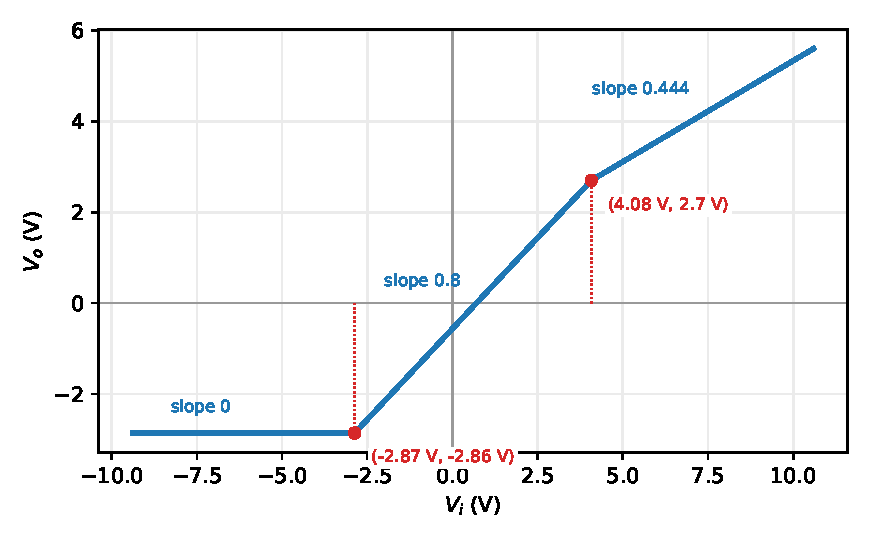
\includegraphics[width=0.62\linewidth,height=6cm,keepaspectratio]{p17_transfer}\end{center}

\begin{ansbox}
$V_o = \begin{cases} -2.857 & V_i < -2.871 \\ 0.8V_i - 0.56 & -2.871 < V_i < 4.075 \\ 0.4444V_i + 0.8889 & V_i > 4.075 \end{cases}$
\end{ansbox}

\newpage
\subsection*{Solution 3A.18 \hfill Hard}
\begin{center}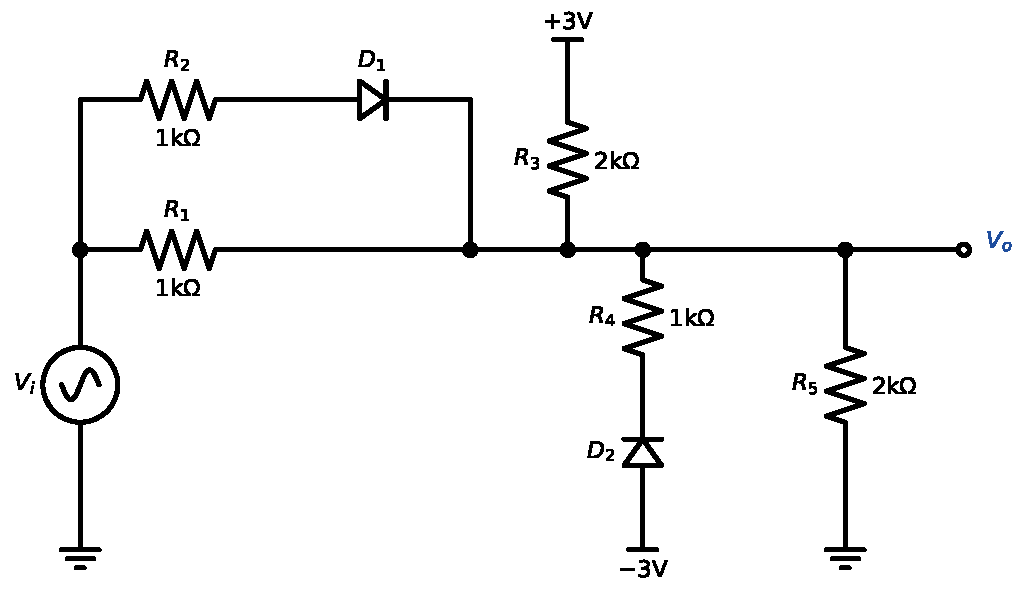
\includegraphics[width=0.9\linewidth,height=5cm,keepaspectratio]{p18_circuit}\end{center}
\solstep{1}{Model and method}Use the constant-voltage-drop model (tool T1): an OFF diode is an open circuit and needs $V_D<0.7$\,V; an ON diode is a $0.7$\,V source and needs $I_D>0$. With 2 diodes there are $4$ ON/OFF combinations. For each one the circuit is linear: solve it with $V_i$ kept as a symbol, then check its assumptions --- each check is a condition on $V_i$ (tool T2). Node names used below: $V_{a}$ = node joining $D_{1}, R_{2}$; $V_{b}$ = node joining $D_{2}, R_{4}$.
\solstep{2}{Assume $D_{1}$ OFF, $D_{2}$ ON}Replace $D_{1}$ OFF: an open circuit; $D_{2}$ ON: a $0.7$\,V source ($-3 - V_{b} = 0.7$) carrying an unknown current $I_{D_{2}}$ from anode to cathode.

Equations (KCL at every node that is not an op-amp output, plus the diode voltages):\begin{align*}
&\text{KCL at }V_{a}: && \frac{V_{a} - V_i}{R_{2}} = 0 \\
&\text{KCL at }V_{b}: && \frac{V_{b} - V_{o}}{R_{4}} - I_{D_{2}} = 0 \\
&\text{KCL at }V_{o}: && \frac{V_{o} - V_i}{R_{1}} + \frac{V_{o} - 3}{R_{3}} + \frac{V_{o} - V_{b}}{R_{4}} + \frac{V_{o}}{R_{5}} = 0 \\
&\text{D2 ON}: && -3 - V_{b} = 0.7
\end{align*}


Solving these linear equations (substitute one into the other, as in Lecture 2) gives, with $V_i$ kept as a symbol:\begin{align*}
V_{o} &= 0.3333V_i - 0.7333 \\
V_{D_{1}} = V_{a} - V_{o} &= 0.6667V_i + 0.7333 \\
I_{D_{2}} &= -0.3333V_i - 2.967\ \mathrm{mA}
\end{align*}


Check the assumptions: $V_{D_{1}} < 0.7$ $\Rightarrow$ $V_i < -0.05$\,V; $I_{D_{2}} > 0$ $\Rightarrow$ $V_i < -8.9$\,V. So this state holds for $\boxed{V_i < -8.9}$, where $V_o = 0.3333V_i - 0.7333$.
\solstep{3}{Assume $D_{1}$ OFF, $D_{2}$ OFF}Replace $D_{1}$ OFF: an open circuit; $D_{2}$ OFF: an open circuit.

Equations (KCL at every node that is not an op-amp output, plus the diode voltages):\begin{align*}
&\text{KCL at }V_{a}: && \frac{V_{a} - V_i}{R_{2}} = 0 \\
&\text{KCL at }V_{b}: && \frac{V_{b} - V_{o}}{R_{4}} = 0 \\
&\text{KCL at }V_{o}: && \frac{V_{o} - V_i}{R_{1}} + \frac{V_{o} - 3}{R_{3}} + \frac{V_{o} - V_{b}}{R_{4}} + \frac{V_{o}}{R_{5}} = 0
\end{align*}


Solving these linear equations (substitute one into the other, as in Lecture 2) gives, with $V_i$ kept as a symbol:\begin{align*}
V_{o} &= 0.5V_i + 0.75 \\
V_{D_{1}} = V_{a} - V_{o} &= 0.5V_i - 0.75 \\
V_{D_{2}} = -3 - V_{b} &= -0.5V_i - 3.75
\end{align*}


Check the assumptions: $V_{D_{1}} < 0.7$ $\Rightarrow$ $V_i < 2.9$\,V; $V_{D_{2}} < 0.7$ $\Rightarrow$ $V_i > -8.9$\,V. So this state holds for $\boxed{-8.9 < V_i < 2.9}$, where $V_o = 0.5V_i + 0.75$.
\solstep{4}{Assume $D_{1}$ ON, $D_{2}$ OFF}Replace $D_{1}$ ON: a $0.7$\,V source ($V_{a} - V_{o} = 0.7$) carrying an unknown current $I_{D_{1}}$ from anode to cathode; $D_{2}$ OFF: an open circuit.

Equations (KCL at every node that is not an op-amp output, plus the diode voltages):\begin{align*}
&\text{KCL at }V_{a}: && \frac{V_{a} - V_i}{R_{2}} + I_{D_{1}} = 0 \\
&\text{KCL at }V_{b}: && \frac{V_{b} - V_{o}}{R_{4}} = 0 \\
&\text{KCL at }V_{o}: && \frac{V_{o} - V_i}{R_{1}} + \frac{V_{o} - 3}{R_{3}} + \frac{V_{o} - V_{b}}{R_{4}} + \frac{V_{o}}{R_{5}} - I_{D_{1}} = 0 \\
&\text{D1 ON}: && V_{a} - V_{o} = 0.7
\end{align*}


Solving these linear equations (substitute one into the other, as in Lecture 2) gives, with $V_i$ kept as a symbol:\begin{align*}
V_{o} &= 0.6667V_i + 0.2667 \\
I_{D_{1}} &= 0.3333V_i - 0.9667\ \mathrm{mA} \\
V_{D_{2}} = -3 - V_{b} &= -0.6667V_i - 3.267
\end{align*}


Check the assumptions: $I_{D_{1}} > 0$ $\Rightarrow$ $V_i > 2.9$\,V; $V_{D_{2}} < 0.7$ $\Rightarrow$ $V_i > -5.95$\,V. So this state holds for $\boxed{V_i > 2.9}$, where $V_o = 0.6667V_i + 0.2667$.
\solstep{5}{The other combinations}\begin{itemize}[leftmargin=*,itemsep=2pt]
\item $D_{1}$ ON, $D_{2}$ ON: $I_{D_{1}}>0$ needs $V_i > -0.05$; $I_{D_{2}}>0$ needs $V_i < -5.95$ --- these cannot all hold, so this state never occurs.
\end{itemize}

\solstep{6}{Assemble and sketch}Put the valid states together:\[
V_o = \begin{cases} 0.3333V_i - 0.7333 & V_i < -8.9 \\ 0.5V_i + 0.75 & -8.9 < V_i < 2.9 \\ 0.6667V_i + 0.2667 & V_i > 2.9 \end{cases}
\]
Check: the pieces must meet at each breakpoint --- at $V_i=-8.9$\,V both pieces give $V_o=-3.7$\,V; at $V_i=2.9$\,V both pieces give $V_o=2.2$\,V. \checkmark\begin{center}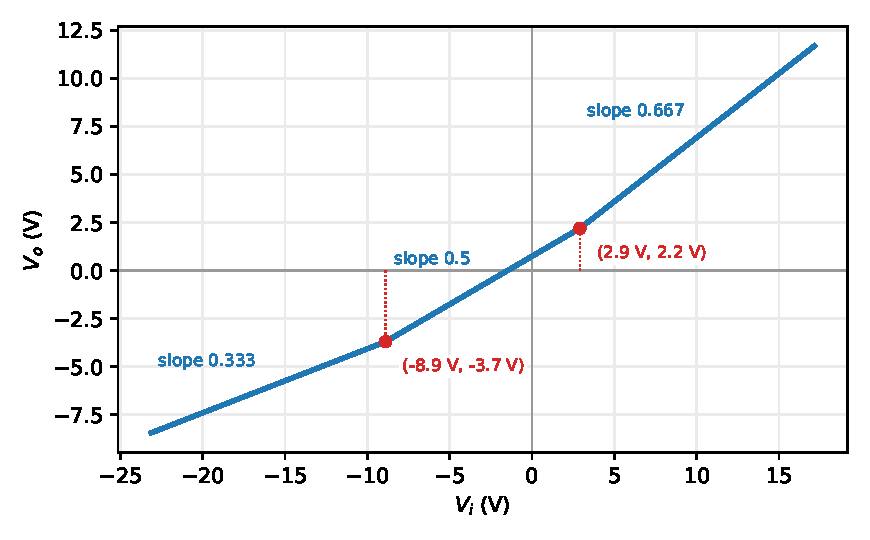
\includegraphics[width=0.62\linewidth,height=6cm,keepaspectratio]{p18_transfer}\end{center}
For $V_i(t) = 8\sin(2\pi\cdot 1000\,t)$ simply pass every instant of $V_i(t)$ through the characteristic above (each piece is a straight line, so each part of the sinusoid is scaled and shifted):\begin{center}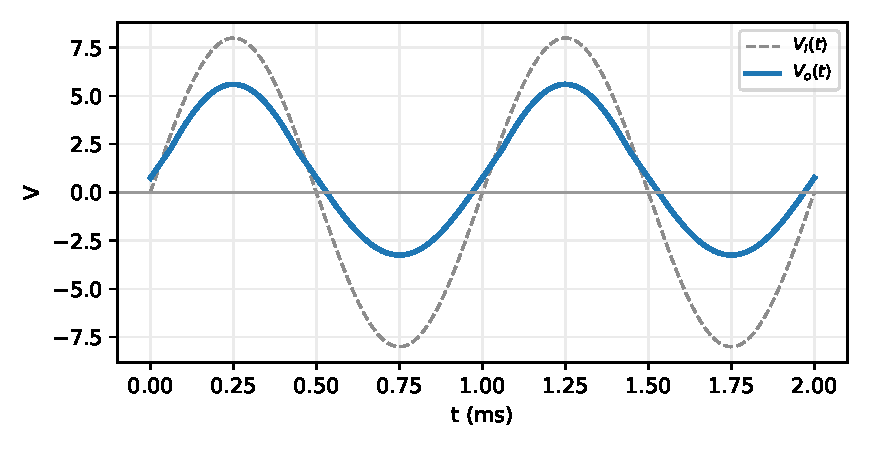
\includegraphics[width=0.62\linewidth,height=5cm,keepaspectratio]{p18_time}\end{center}

\begin{ansbox}
$V_o = \begin{cases} 0.3333V_i - 0.7333 & V_i < -8.9 \\ 0.5V_i + 0.75 & -8.9 < V_i < 2.9 \\ 0.6667V_i + 0.2667 & V_i > 2.9 \end{cases}$
\end{ansbox}

\end{document}
